\documentclass[12pt]{article}

\usepackage{sbc-template}


\usepackage{graphicx,url,tabularx,multirow,multicol,booktabs}
\usepackage{amssymb,amsmath,latexsym,mathabx,wasysym,stmaryrd}
\usepackage[brazil]{babel}
\usepackage[utf8]{inputenc} 
\usepackage{colortbl}

\sloppy

%\title{Inferência de Desempenho: Uma Nova Abordagem para Planejar a Capacidade de Aplicações na Nuvem}
\title{Inferência de Desempenho: Uma Nova Abordagem para o Planejamento da Capacidade de Aplicações na Nuvem}
\author{Marcelo Gonçalves, Matheus Cunha, Américo Sampaio, Nabor C. Mendonça}

\address{Programa de Pós-Graduação em Informática Aplicada (PPGIA)\\
Universidade de Fortaleza (UNIFOR)\\
Av. Washington Soares, 1321, Edson Queiroz, CEP 60811-905 Fortaleza, CE
\email{\{marcelocg,mathcunha\}@gmail.com,\{americo.sampaio,nabor\}@unifor.br}
}

\begin{document} 

\maketitle

\begin{resumo} 

%Um dos principais desafios enfrentados pelos usuários de nuvens que oferecem infraestrutura- como-serviço (IaaS) é planejar adequadamente a capacidade dos recursos da nuvem necessários às suas aplicações. 

Este trabalho propõe uma nova abordagem para apoiar o planejamento da capacidade de aplicações em nuvens que oferecem infraestrutura-como-serviço (IaaS). A abordagem proposta tem como premissa a existência de uma relação de capacidade entre diferentes configurações de recursos de um dado provedor de nuvem IaaS, com a qual é possível prever (ou ``inferir''), com alta precisão, o desempenho esperado de uma aplicação para certas configurações de recursos e cargas de trabalho, tendo com base o desempenho da aplicação observado para outras configurações de recursos e cargas de trabalho neste mesmo provedor. Resultados empíricos preliminares, obtidos a partir da avaliação do desempenho de uma popular aplicação de \emph{blogging} (WordPress) em um provedor de nuvem público (Amazon EC2), mostram que a nova abordagem consegue reduzir significativamente (acima de 80\%) o número total de cenários de implantação da aplicação que precisam de fato ser avaliados na nuvem.

\end{resumo}

\begin{abstract}

%One of the main challenges faced by users of infrastructure-as-a-service (IaaS)  clouds is to adequately plan the cloud resources required to the meet their applications' needs. 

This work proposes a novel approach to support application capacity planning in infrastructure-as-a-service (IaaS) clouds. The proposed approach relies on the assumption that there exists a capacity relation between different resource configurations offered by a given IaaS cloud provider, enabling one to predict (or ``infer''), with high accuracy, an application's expected performance for certain resource configurations and workloads, based upon its observed performance for other resource configurations and workloads in that same provider. Preliminary empirical results, obtained from evaluating the performance of a well-known blogging application (WordPress) in a public cloud provider (Amazon EC2), show that the proposed approach can significantly reduce (over 80\%) the total number of application deployment scenarios that need to be effectively tested in the cloud.

\end{abstract}

\section{Introdução}\label{sec:introducao}

%A computação em nuvem é um paradigma computacional que está transformando a forma de desenvolver e gerenciar aplicações e serviços de Tecnologia da Informação \cite{Murugesan2014}. Diversas organizações passaram a adotar este paradigma atraídas pelo seu modelo de negócios onde recursos computacionais (ex.: computação, armazenamento e transferência de dados) podem ser consumidos, sob-demanda, como um serviço e pagos de acordo com o consumo efetuado. 

Um dos principais desafios enfrentados pelos usuários de nuvens que oferecem infraestrutura-como-serviço (IaaS) é a planejar adequadamente a capacidade dos recursos da nuvem necessários para atender as demandas específicas de suas aplicações \cite{Menasce2009}.  Parte desse desafio envolve tentar descobrir a melhor maneira de implantar a aplicação na nuvem, considerando os vários tipos de recursos (em particular, máquinas virtuais) oferecidos pelo provedor, sob a perspectiva de diferentes requisitos e critérios de qualidade \cite{GoncalvesJunior2015}.  

Em geral, provedores de nuvens IaaS cobram seus usuários em função do tempo de utilização dos recursos solicitados, cujos preços variam conforme a capacidade (normalmente medida por características técnicas como quantidade de núcleos de processamento, tamanho de memória e espaço de armazenamento) de cada recurso. Dessa forma, para calcular o custo de operação de uma aplicação na nuvem, é preciso estimar ou medir como a aplicação responderá a diferentes níveis de demanda, em termos de indicadores de desempenho como tempo de resposta ou vazão, quando executada sob diferentes configurações e perfis de máquinas virtuais. Na prática, isso significa que cabe ao usuário da nuvem identificar, dentre as possíveis configurações de máquinas virtuais ofertadas por um ou mais provedores de nuvem, aquelas de menor custo capazes de executar a aplicação mantendo-se níveis satisfatórios para os indicadores de desempenho.

% ... Somem-se a isso as inúmeras possibilidades de implantação da aplicação considerando tanto estratégias de escalabilidade vertical (variando-se a quantidade de recursos de cada máquina) quanto horizontal (variando-se a quantidade de máquinas em uma ou mais camadas da aplicação, como dados, apresentação e negócio), chega-se a um conjunto bastante amplo de cenários de implantação a serem investigados. 

%Outro desafio ao planejamento de capacidade decorre da constatação de que configurações formadas por recursos com perfis similares, ainda que do mesmo provedor, podem responder de maneira diferente quando submetidas a um mesmo nível de carga de trabalho, a depender do momento em que sejam utilizadas \cite{cunha2011investigating, iosup2011performance, jayasinghe2011variations}. Independente do motivo que leve a esse comportamento de certa forma imprevisível, é preciso levar em conta nos testes de avaliação de desempenho essa variabilidade, o que pode pode ser alcançado através da repetição dos cenários de teste em horários e dias diferentes.

Um grande problema começa a se desenhar para o usuário da nuvem ao seguir essa abordagem: a fase de avaliação da aplicação pode atingir patamares elevados de tempo e custo, em razão das necessidades de variação da demanda, da arquitetura de implantação e das configurações de recursos utilizadas para hospedar cada camada da aplicação \cite{silva2013cloudbench}. Ainda que certos provedores IaaS ofereçam descontos ou pacotes de horas grátis para novos clientes, em geral esses incentivos, por estarem limitados a máquinas de pequeno porte, são insuficientes para suportar a carga de uma aplicação real em produção. Assim, executar uma aplicação real, tipicamente implantada em arquitetura de várias camadas~\cite{jayasinghe2011variations}, em máquinas virtuais de tamanho considerável e por longos períodos de tempo, apenas para estudar o seu comportamento, pode se traduzir em um custo alto que dificulte ou até mesmo inviabilize o próprio projeto de migração dessa aplicação para a nuvem~\cite{beserra2012cloudstep}. 

Vários trabalhos já foram propostos com o intuito de apoiar o planejamento da capacidade de aplicações em nuvens IaaS. Em linhas gerais, esses trabalhos podem ser classificados de acordo duas abordagens distintas quanto à estratégia de avaliação do desempenho da aplicação. Trabalhos que seguem a primeira abordagem, referenciada neste trabalho como \emph{abordagem preditiva}, visam estimar ou simular o desempenho esperado da aplicação para determinadas configurações de recursos e determinados níveis\l de carga, sem necessariamente ter que implantá-la na nuvem  \cite{cloudharmony, malkowski2010cloudxplor, fittkau2012cdosim, li2011cloudprophet, jung2013cloudadvisor}. Apesar do baixo custo oferecido aos usuários, que não precisam pagar por recursos de nuvem durante a fase de avaliação, esse trabalhos têm como maior limitação a ainda baixa precisão das técnicas de predição de desempenho, particularmente daquelas baseadas em simulação~\cite{fittkau2012cdosim}. Já os trabalhos que fazem parte da segunda abordagem, aqui referenciada como \emph{abordagem empírica}, tem como objetivo medir o desempenho real da aplicação através de sua efetiva implantação na nuvem e da realização de testes de carga \cite{jayasinghe2012, silva2013cloudbench, cunha2013b, scheuner2014cloud}. Por executarem a aplicação no próprio ambiente de nuvem, esses trabalhos conseguem resultados significativamente mais precisos no que diz respeito à seleção das melhores configurações de recursos para cargas de trabalho específicas. No entanto, uma limitação importante desses trabalhos é a necessidade de se testar exaustivamente uma grande quantidade de configurações de recursos e cargas de trabalho, implicando em altos custos durante a fase de avaliação. 

%As técnicas de predição de desempenho adotadas na abordagem preditiva variam conforme o trabalho, sendo as mais comuns o uso de simuladores \cite{fittkau2012cdosim} e a analogia com resultados previamente obtidos através da utilização de \emph{benchmarks} \cite{cloudharmony, malkowski2010cloudxplor}. Apesar do baixo custo oferecido aos usuários, que não precisam pagar por recursos de nuvem durante a fase de avaliação, trabalhos da abordagem preditiva têm como maior limitação uma ainda baixa precisão na sua  capacidade de prever o desempenho da aplicação alvo. Isto se deve principalmente a diferenças conceituais entre o ambiente da nuvem real e os modelos de simulação \cite{fittkau2012cdosim}, ou à ausência de \emph{benchmarks} com comportamento e perfis de carga de trabalho similares aos da aplicação alvo. Já os trabalhos que utilizam a abordagem empírica, por executarem a aplicação no próprio ambiente de nuvem, conseguem obter resultados significativamente mais precisos no que diz respeito à seleção das melhores configurações de recursos para cargas de trabalho específicas. No entanto, uma limitação importante desses trabalhos é a necessidade de se testar exaustivamente uma grande quantidade de configurações de recursos e cargas de trabalho, implicando em altos custos durante a fase de avaliação.

Visando combinar as vantagens das abordagens preditiva e empírica, este trabalho propõe uma nova maneira de apoiar os usuários de nuvens IaaS a identificarem as melhores (i.e., mais baratas) configurações de recursos capazes de satisfazer as demandas específicas de suas aplicações. A nova abordagem tem como premissa a existência de uma relação de capacidade entre diferentes configurações de recursos oferecidas por um dado provedor de nuvem, com a qual é possível prever (ou ``inferir''), com alta precisão, o desempenho esperado da aplicação para determinadas configurações de recursos. A predição ou inferência é realizada com base no desempenho observado da aplicação para outras configurações de recursos e cargas de trabalho no mesmo provedor. Por exemplo, se a aplicação atendeu satisfatoriamente a demanda para uma configuração de recursos de determinada capacidade sob um determinada carga de trabalho, é muito provável que ela também vá atendê-la para outras configurações de maior capacidade sob a mesma carga de trabalho. Analogamente, se a aplicação não atendeu a demanda para uma determinada configuração de recursos sob uma determinada carga de trabalho, muito provavelmente ela também não irá atendê-la para a mesma configuração sob cargas de trabalho maiores. Através do uso de inferência, a abordagem permite avaliar uma ampla variedade de cenários de implantação da aplicação, sendo que apenas uma pequena parte desses cenários precisa de fato ser implantada e executada na nuvem. Dessa forma, a abordagem consegue obter o melhor das duas abordagens previamente citadas, produzindo resultados de alta precisão (característicos da abordagem empírica) mas com significativa redução de custo (característica da abordagem preditiva).

A próxima seção apresenta um novo processo de avaliação de capacidade para aplicações na nuvem, fundamentado no conceito de inferência de desempenho. A Seção~\ref{sec:experiments} descreve os resultados de uma avaliação preliminar do novo processo envolvendo a implantação de uma aplicação real (WordPress) em um provedor de nuvem IaaS público (Amazon EC2). A Seção~\ref{sec:related-work} compara o novo processo com outros trabalhos relacionados. Por fim, a Seção~\ref{sec:conclusion} oferece algumas conclusões e sugestões para trabalhos futuros.


\section{Processo de Avaliação de Capacidade por Inferência de Desempenho}\label{sec:process}

\subsection{Conceitos e Terminologia}

Antes de apresentarmos o processo, é necessário definirmos alguns conceitos importantes relacionados ao domínio da avaliação da capacidade de aplicações na nuvem (ver \mbox{Tabela~\ref{tab:concepts}}). A definição desses conceitos também serve para estabelecer a terminologia que será utilizada na descrição do processo, feita a seguir.

\begin{table}[t*]
\centering\scriptsize
\caption{Conceitos e terminologia utilizados no artigo.}
\label{tab:concepts}
%\tabsize
%\begin{tabularx}{\linewidth}{|l|X|}
\begin{tabularx}{\linewidth}{lX}
%\hline
\toprule
%\multicolumn{1}{|c|}\textbf{Conceito}} & \multicolumn{1}{c|}{\textbf{Definição}} \\
\multicolumn{1}{c}{\textbf{Conceito}} & \multicolumn{1}{c}{\textbf{Definição}} \\
%\hline
\midrule
\emph{Aplicação sob teste} & Um sistema computacional, possivelmente implementado em uma arquitetura multicamadas, para o qual se deseja observar o comportamento em um ambiente de computação em nuvem e ao qual estão associadas uma ou mais {\em métricas de desempenho}.
\\[0.03cm]%\hline
\emph{Métrica de desempenho} &
Uma característica ou comportamento mensurável de forma automatizada e comparável a um {\em valor de referência}, capaz de indicar o grau de sucesso de uma execução da aplicação sob teste. É dependente do domínio da aplicação. Ex.: tempo de resposta, quadros por segundo.
\\[0.03cm]%\hline
\emph{Valor de referência (SLA)} &
Um valor predefinido como minimamente aceitável  para uma métrica de desempenho após uma execução da aplicação sob teste. Este valor, também referenciado neste trabalho como SLA (\emph{Service Level Agreement}), serve como base de comparação para que se classifique a aplicação como capaz de ser executada em uma certa {\em configuração} de máquinas virtuais e sob uma certa {\em carga de trabalho}.
\\[0.03cm]%\hline
\emph{Provedor} &
Uma empresa que fornece recursos computacionais como serviço cobrado financeiramente por fração de tempo de utilização. Neste trabalho, o foco será em provedores que disponibilizam recursos de infraestrutura, notadamente {\em máquinas virtuais}.
\\[0.03cm]%\hline
\emph{Tipos de máquinas virtuais} &
Classificam as máquinas virtuais fornecidas por um provedor conforme suas características técnicas (e.g., núcleos de processamento, tamanho de memória, espaço em disco), permitindo que o provedor mantenha uma linha de produtos discreta e finita.
\\[0.03cm]%\hline
\emph{Categorias} &
Agrupam os tipos de máquinas virtuais de um provedor de acordo com suas características técnicas, plataforma e/ou arquitetura de hardware e a natureza do uso a que se destinam. Ex.: categorias que priorizam consumo de memória, acesso a disco, processamento gráfico, etc. 
\\[0.03cm]%\hline
\emph{Configuração} &
Um conjunto de máquinas virtuais de um mesmo tipo e, portanto, de uma mesma categoria. {\em Configurações} são usadas para implantar uma ou mais camadas arquiteturais (ex.: apresentação, negócio, persistência) da aplicação sob teste.
\\[0.03cm]%\hline
\emph{Espaço de implantação} &
Denota um conjunto limitado de configurações de máquina virtuais nas quais a aplicação sob teste será implantada e executada durante uma sessão de avaliação. 
\\[0.03cm]%\hline
\emph{Relações de capacidade} &
Relativizam o poder computacional das diversas configurações que compõem o espaço de implantação. As {\em relações de capacidade} definem um grafo orientado sobre o espaço de implantação onde os vértices correspondem às configurações e as arestas indicam a superioridade ou inferioridade (dependendo da direção da aresta) de uma configuração em relação a outra em termos de poder computacional.  
\\[0.03cm]%\hline
\emph{Níveis de capacidade} &
Estabelecem uma hierarquia sobre as relações de capacidade definidas entre as configurações do espaço de implantação. Nessa hierarquia, configurações classificadas em um mesmo nível de capacidade seriam equivalentes (ou indistinguíveis) em termos de poder computacional. 
\\[0.03cm]%\hline
\emph{Carga de trabalho} &
Representa o tamanho da demanda que será imposta à aplicação sob teste em uma execução. Sua unidade de medida é dependente do domínio da aplicação. Ex.: tamanho dos arquivos de entrada para uma aplicação de compactação de arquivos, quantidade de usuários concorrentes para uma aplicação web, etc.
\\[0.03cm]%\hline
\emph{Execução} &
Corresponde à execução da aplicação sob teste utilizando uma determinada configuração de máquinas virtuais e submetida a uma determinada carga de trabalho. O resultado de uma {\em execução} fornece indicadores que permitirão avaliar se a aplicação atingiu o valor de referência esperado para uma determinada métrica de desempenho naquele cenário.
\\%\hline
\bottomrule
\end{tabularx}
\end{table}

%\subsection{Visão Geral do Processo}
%
%O processo de avaliação de capacidade proposto neste trabalho prevê um conjunto de dados de entrada, uma ou mais execuções da aplicação sob teste no ambiente de nuvem almejado para hospedá-la, e a análise do desempenho obtido pela aplicação a partir dos resultados de suas execuções, como ilustra a Figura~\ref{fig:fig_processo_alto_nivel}. Com base nos dados de desempenho, o processo passa por diversos pontos de decisão que podem levar a novas execuções da aplicação utilizando diferentes configurações de máquinas virtuais e sob diferentes níveis de carga. Ao final do processo, é fornecida como saída uma lista de configurações, ordenadas por preço, capazes de obter o desempenho esperado da aplicação para cada nível de carga avaliado.
%
%\begin{figure}[t]
%  \begin{center}
%   %trim option's parameter order: left bottom right top
%    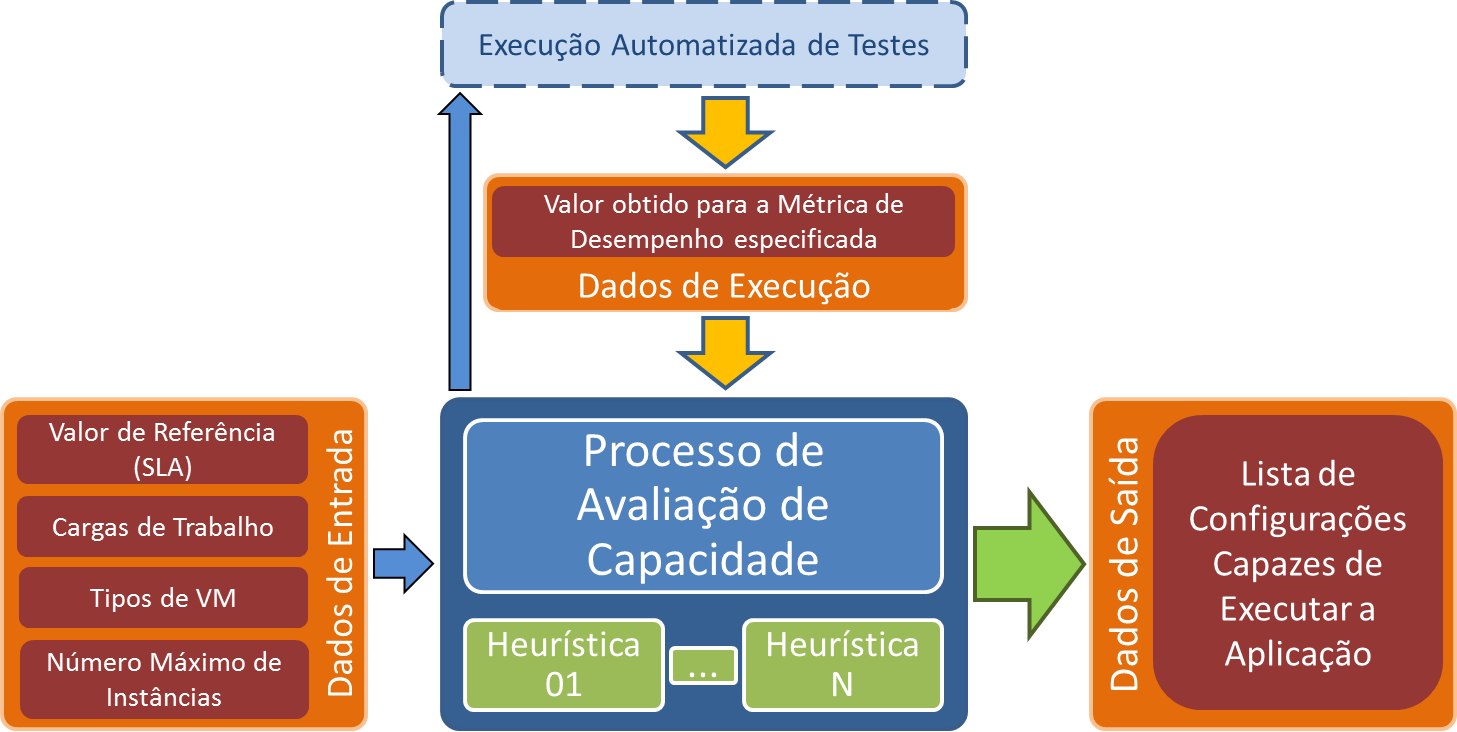
\includegraphics[trim = 20mm 5mm 20mm 5mm, scale=0.4]{img/processoAltoNivel}
%  \end{center}
%  \caption{\label{fig:fig_processo_alto_nivel}Visão geral do processo de  avaliação de capacidade.}
%\end{figure}

%O restante desta seção aborda em detalhes todas as etapas do processo proposto, explicando quais são os dados recebidos como entrada, as diferentes atividades executadas e as decisões a serem tomadas para que o processo possa determinar as configurações que atendem os requisitos de desempenho e carga de trabalho da aplicação.

\subsection{Dados de Entrada}

O principal dado de entrada esperado pelo processo é o valor de referência (SLA), o qual será usado para determinar 
se a aplicação atingiu os requisitos mínimos de desempenho exigidos em cada cenário de execução. Além do SLA, o processo precisa também conhecer quais são as cargas de trabalho sob as quais o desempenho da aplicação deverá ser avaliado. Outro dado importante que deve ser passado como entrada para o processo é o espaço de implantação da aplicação. Para isso, o processo deve ser alimentado com três parâmetros: (i) uma lista de tipos de máquinas virtuais fornecidos pelo provedor no qual deseja-se hospedar a aplicação; (ii) a quantidade máxima de máquinas virtuais de cada tipo que irá compor cada configuração a ser avaliada; e (iii) um critério para estabelecimento das relações de capacidade entre as configurações do espaço de implantação. 

Para dar um exemplo de como os três parâmetros acima são utilizados na construção do espaço de implantação, considere que o processo recebeu um único tipo de máquina virtual; o valor 3 como sendo a quantidade máxima de máquinas virtuais por configuração; e a quantidade de máquinas virtuais de cada configuração como critério para estabelecimento das relações de capacidade. Nesse caso, o espaço de implantação seria composto por 3 configurações distintas, contendo 1, 2 e 3 máquinas do tipo passado como parâmetro, respectivamente. Além disso, configurações maiores (ou seja, contendo um maior número de máquinas virtuais) seriam classificadas acima de configurações menores na hierarquia de níveis de capacidade estabelecida sobre o espaço de implantação.


%\begin{figure}[t]
%  \begin{center}
%    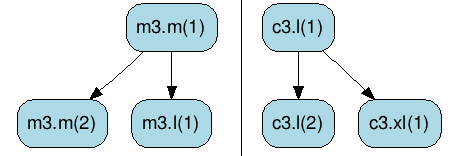
\includegraphics[scale=.5]{img/exemplo-niveis-capacidade}
%  \end{center}
%  \caption{\label{fig_niveis_capacidade}Exemplo de relações e níveis de capacidade entre configurações.}
%\end{figure}
%
%A Figura~\ref{fig_niveis_capacidade} mostra um pequeno exemplo de um espaço de implantação, no qual 6 configurações,
%pertencentes a duas categorias distintas, foram classificadas em dois níveis de capacidade dentro de cada categoria. Nesse exemplo, os retângulos representam as configurações, com o rótulo de cada retângulo indicando o tipo e a quantidade de máquinas virtuais que compõem a configuração, e as setas que ligam as configurações representam a existência de uma relação de capacidade elas. A ausência de seta entre duas configurações implica a impossibilidade de se estabelecer uma relação de capacidade entre elas. 


\subsection{Atividades}

\begin{figure}[t]
  \begin{center}
    %trim option's parameter order: left bottom right top
    %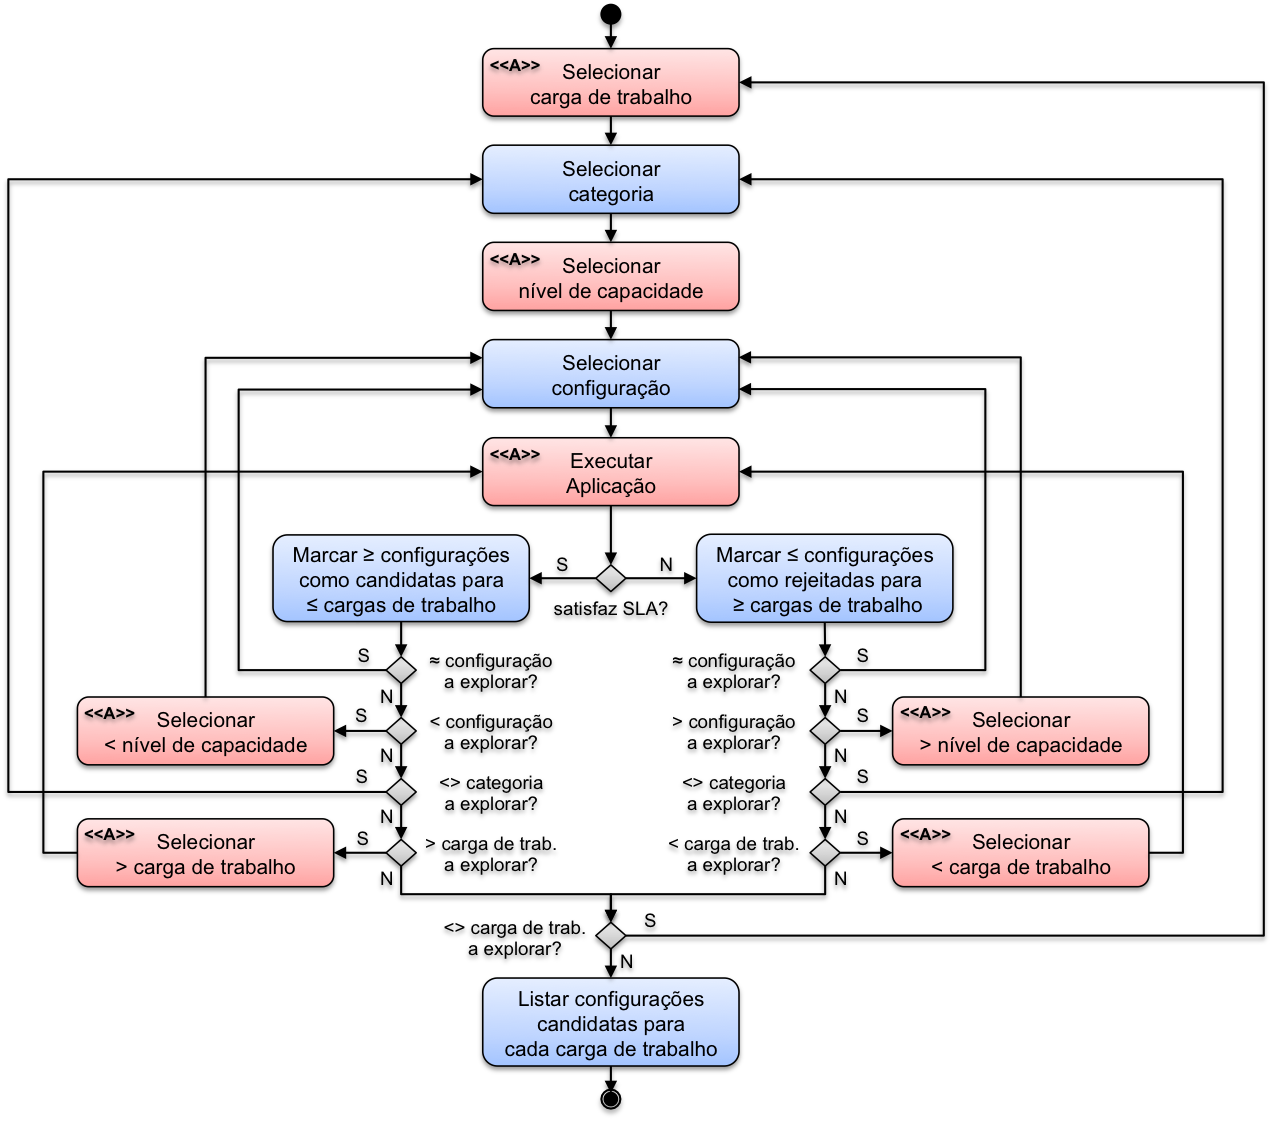
\includegraphics[trim = 20mm 15mm 20mm 25mm, scale=.5]{img/capacity-planning-diagram-v13-1-color-por}
    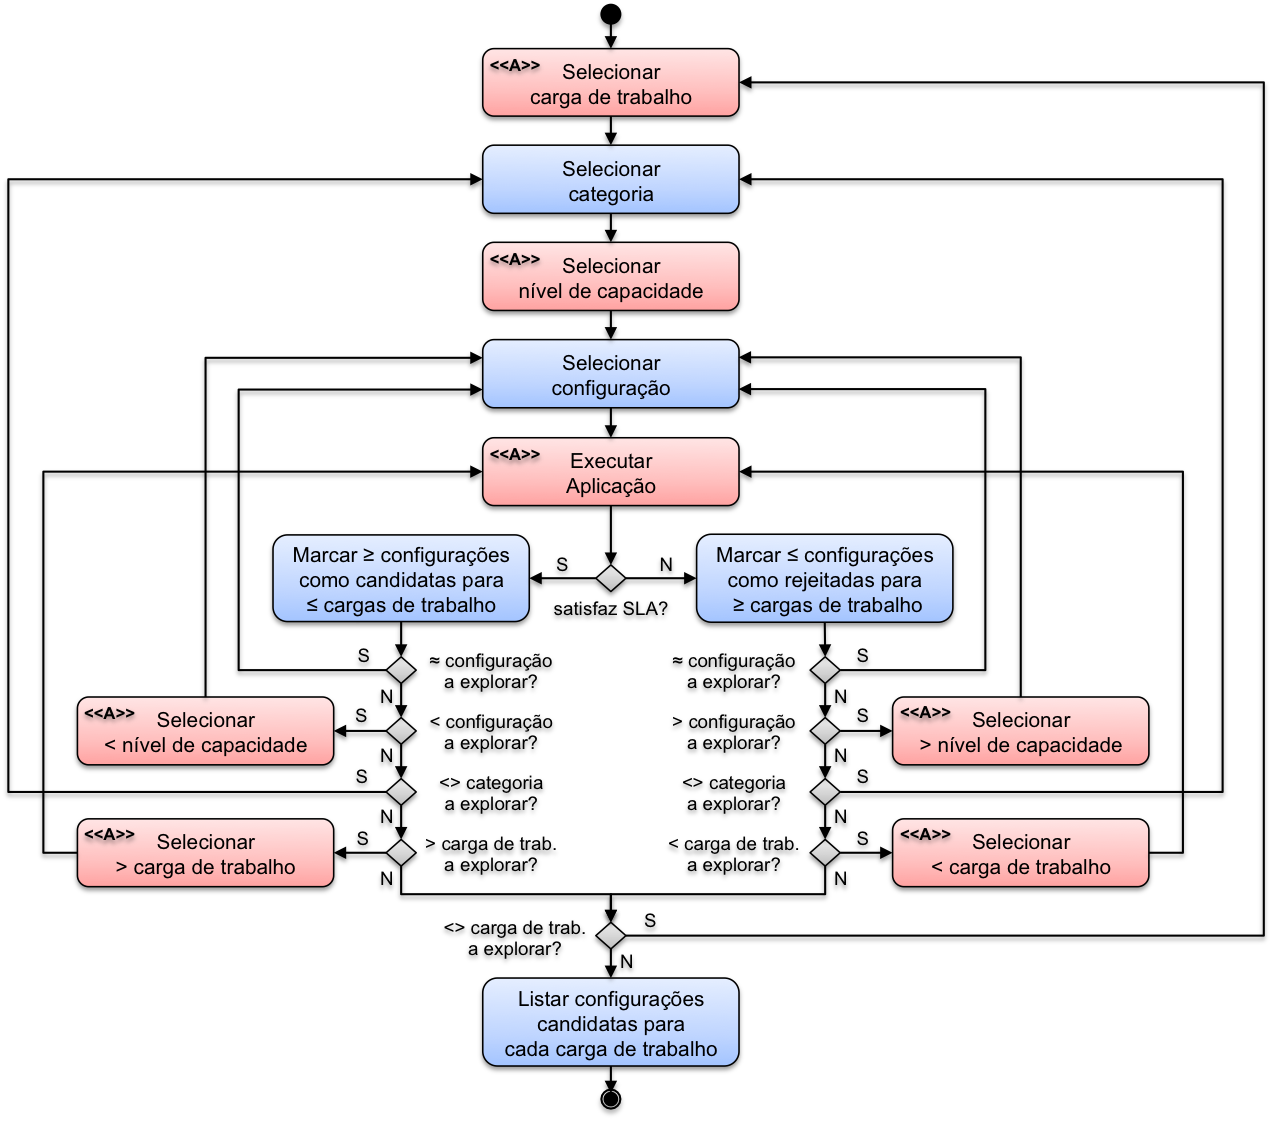
\includegraphics[trim = 20mm 6mm 20mm 5mm, scale=.65]{img/capacity-planning-diagram-v13-1-color-por}
    %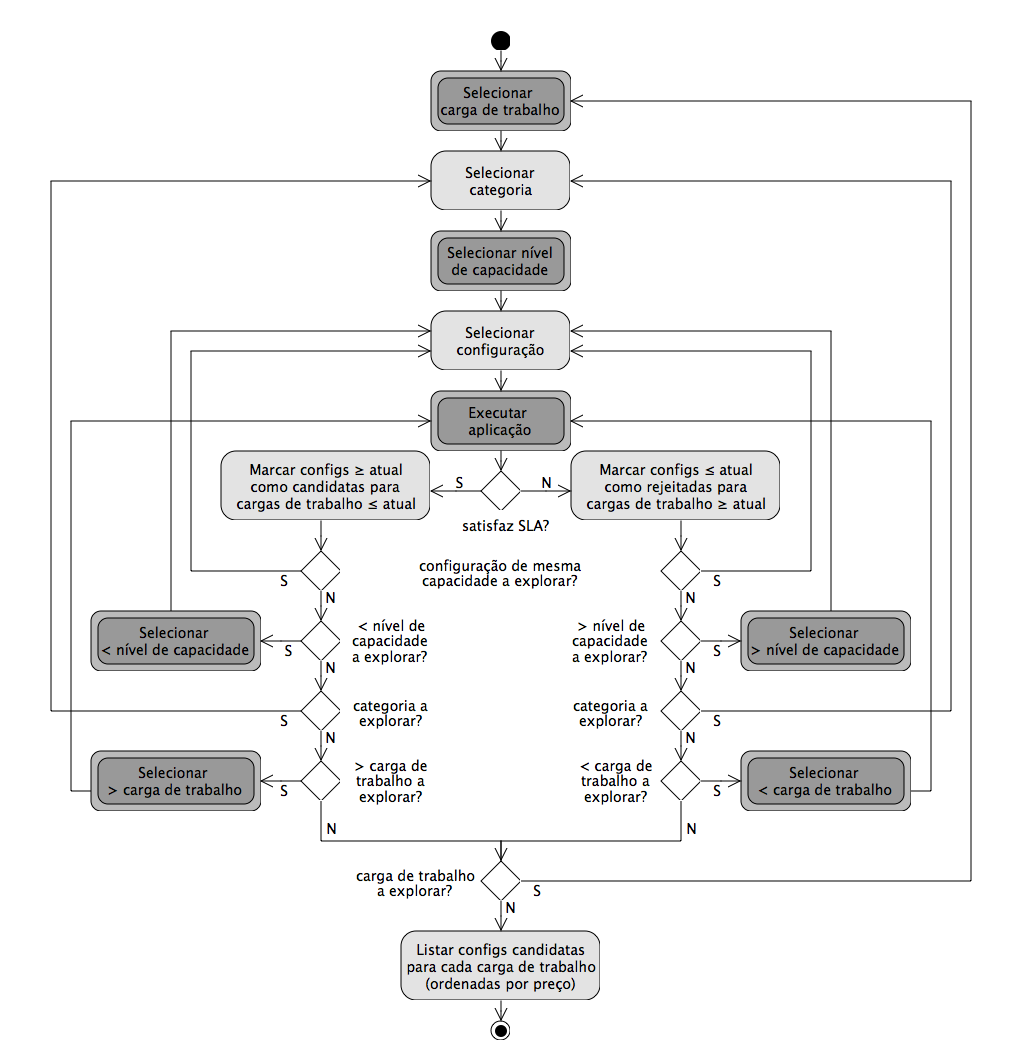
\includegraphics[width=\linewidth]{img/capacity-planning-diagram-v13-1-mono-por}
  \end{center}
  \caption{\label{fig:fig_processo_aval_capacidade}Diagrama de atividades do processo de avaliação de capacidade.}
\end{figure}


As principais atividades executadas pelo processo de avaliação de capacidade são ilustradas no diagrama da Figura~\ref{fig:fig_processo_aval_capacidade}. As atividades destacas com o rótulo ``\mbox{\boldmath$\ll${\sc a}$\gg$}'' são atividades abstratas, devendo ser customizadas pelos usuários do processo de acordo com diferentes estratégias de avaliação (descritas na seção~\ref{sec:strategies}). As outras atividades são executadas de maneira idêntica independentemente de qual seja a aplicação sob teste ou de qual seja a estratégia de avaliação utilizada. 

A execução do processo acontece em quatro fases bem distintas e cíclicas: seleção do cenário de execução da aplicação; execução da aplicação; inferência de desempenho; e seleção do próximo cenário. Cada uma dessas fases será detalhada a seguir.

\subsubsection{Seleção do cenário de execução}

A primeira atividade dessa fase é a escolha de uma carga de trabalho. Essa é uma atividade abstrata, significando que diferentes estratégia podem ser empregadas nessa escolha, por exemplo, selecionando um carga de trabalho maior ou menor dentre aquelas fornecidas como dados de entrada ao processo. Depois de selecionar a carga inicial, o processo seleciona uma categoria de máquinas virtuais. No caso da categoria, a ordem ou método utilizado na escolha é irrelevante para o processo, uma vez que todas as categorias do espaço de implantação deverão ser avaliadas. Em seguida, o processo seleciona um nível de capacidade dentre aqueles presentes no espaço de implantação. Essa também é uma atividade abstrata, uma vez que níveis de capacidade mais acima ou mais abaixo na hierarquia podem ser escolhidos, a depender da estratégia de avaliação utilizada. Por fim, o processo seleciona uma configuração do nível de capacidade previamente selecionado. A ordem de seleção das configurações também é irrelevante, uma vez que todas as 
configurações daquele nível de capacidade devem ser avaliadas. 

\subsubsection{Execução da aplicação}

Uma vez escolhidos uma carga de trabalho, uma categoria, um nível de capacidade e uma configuração, o processo está apto a executar a aplicação na nuvem. A execução da aplicação também é uma atividade abstrata do processo, pois depende de uma série de fatores que são específicos de cada aplicação ou plataforma de nuvem, como as tecnologias necessárias parar implantar os componentes da aplicação na nuvem bem como para submetê-los aos níveis de carga de trabalho desejados.  Após a execução da aplicação, o processo analisa o resultado obtido e passa para a fase de inferência de desempenho.

\subsubsection{Inferência de desempenho}

Nesta fase, o processo se bifurca, atingindo seu primeiro ponto de decisão. A partir da análise do resultado da execução, que é feita comparando-se os indicadores obtidos para a métrica de desempenho utilizada frente ao valor de referência (SLA) desejado, o processo determina se a aplicação é ou não capaz de atender à demanda imposta sobre ela com a atual configuração. Se a aplicação satisfaz o SLA, o processo assinala a configuração atual como uma {\em configuração candidata} para o atual nível de carga. Do contrário, o processo assinala a configuração atual como uma {\em configuração rejeitada} para esse nível de carga.

É neste momento que a abordagem de inferência de desempenho, proposta originalmente neste trabalho, entra em ação. Com base nas relações de capacidade presentes no espaço de implantação, o processo pode ``inferir'' o provável desempenho da aplicação para outras configurações e cargas de trabalho ainda não avaliadas. Ora, se o processo identificou que uma certa configuração consegue satisfazer a demanda imposta à aplicação sob uma certa carga de trabalho, intuitivamente qualquer outra configuração de maior poder computacional também será capaz de fazê-lo sob a mesma carga de trabalho. Similarmente, é intuitivo concluir que a mesma configuração também será capaz de satisfazer o SLA da aplicação sob cargas de trabalho menores. Assim, usando as informações sobre as relações de capacidade existentes entre as configurações do espaço de implantação, o processo também assinala como candidatas para o atual nível de carga todas as outras configurações identificadas como sendo de ``maior capacidade'' que a configuração atual de acordo com o espaço de implantação. Da mesma forma, o processo também assinala a configuração atual como candidata para todos os níveis de carga inferiores ao nível de carga atual.

O caso em que a configuração atual não satisfaz o SLA  da aplicação é tratado de modo análogo. Nesse caso, o processo assinala como rejeitadas para o atual nível de carga todas as outras configurações identificadas como sendo de ``menor capacidade'' que a configuração atual de acordo com o espaço de implantação. O mesmo acontece com a configuração atual, que também é assinalada como rejeitada para todos os outros níveis de carga superiores ao nível de carga atual.


%\begin{figure}[t]
%  \begin{center}
%    %trim option's parameter order: left bottom right top
%    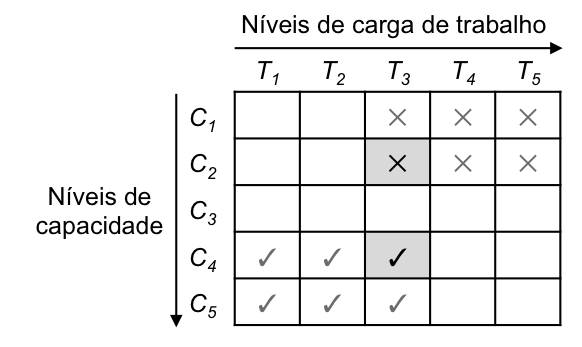
\includegraphics[trim = 20mm 5mm 20mm 5mm, scale=.6]{img/inferencia}
%  \end{center}
%  \caption{\label{fig:fig_processo_inferencia}Ilustração da marcação de configurações como {\em candidatas} (embaixo à esquerda) ou {\em rejeitadas} (no alto à direita) via inferência de desempenho.}
%\end{figure}
%
%O efeito da inferência de desempenho pode ser melhor visualizado através do exemplo de espaço de implantação mostrado na Figura~\ref{fig:fig_processo_inferencia}. Nesse exemplo, o espaço de implantação está representado na forma de uma matriz, cujas linhas correspondem às configurações e as colunas correspondem às cargas de trabalho. Note que o nível de capacidade das configurações cresce de cima para baixo na matriz, enquanto o tamanho da carga de trabalho cresce da esquerda para a direita. A parte inferior esquerda da matriz ilustra o caso em que o SLA é satisfeito em um determinado cenário de execução. Já a parte superior direita ilustra o caso oposto. As células marcadas com um ``{\scriptsize \raisebox{0.4ex}{\boldmath$\surd{}\,$}}'' (``\boldmath$\times{}$'') indicam as configurações marcadas como candidatas (rejeitadas) para as respectivas cargas de trabalho. As duas células em destaque correspondem a execuções reais da aplicação, cujos resultados serviram de base para a inferência do desempenho da aplicação nos outros cenários. 
%
%Esse exemplo é representativo do grande potencial da abordagem de inferência de desempenho para reduzir os custos associados ao processo de planejamento de capacidade, tonando-o mais rápido e eficiente. Note que, considerando os dois casos ilustrados, o processo teria obtido resultados relativos à avaliação de 12 cenários de execução distintos, dos quais apenas dois teriam de fato sido executados na nuvem, o que representa uma economia de quase 90\% em relação à abordagem empírica tradicional, onde todos os cenários de interesse devem ser sistematicamente avaliados.

%Na seção~\ref{sec:experiments}, apresentaremos resultados obtidos empiricamente mostrando que a abordagem de inferência de desempenho consegue prever o desempenho esperado de uma aplicação na nuvem com alta precisão. 

\subsubsection{Seleção do próximo cenário}

Após a fase de inferência de desempenho, o processo seleciona os elementos que comporão o próximo cenário de execução a ser avaliado, ou encerra sua execução, caso não haja mais cenários a explorar. Nesse caso, o processo produz, como saída, uma lista contendo todas as configurações assinaladas como candidatas para cada carga de trabalho avaliada, em ordem crescente de preço.

A seleção do próximo cenário inclui a escolha de uma nova configuração do atual nível de capacidade, a escolha de um novo nível de capacidade (que deverá ser maior ou menor que o nível de capacidade atual, a depender do resultado da execução da aplicação no atual cenário), a escolha de uma nova categoria, ou a escolha de uma nova carga de trabalho (que também deverá ser maior ou menor que o nível de carga atual, novamente a depender do resultado da execução da aplicação no atual cenário). As escolhas do novo nível de capacidade e da nova carga de trabalho também são atividades abstratas, a serem definidas de acordo com a estratégia de avaliação utilizada para customizar o processo. 


\subsection{Estratégias de Avaliação}\label{sec:strategies}

Conforme mencionado anteriormente, todas as atividades abstratas do processo (com exceção da atividade de execução da aplicação na nuvem) devem ser customizadas de acordo com diferentes estratégias de avaliação. Essas atividades incluem, basicamente, a escolha de cargas de trabalho e níveis de capacidade. Tais escolhas influenciam diretamente a maneira através da qual o processo explora o espaço de implantação, tendo um forte impacto no alcance da inferência de desempenho. 

Como exemplo, considere o caso de um espaço de implantação onde nenhuma configuração é capaz de atender a demanda da aplicação sob qualquer nível de carga. Nesse caso, iniciar o processo de avaliação pelas configurações do nível de capacidade mais baixo sob cargas de trabalho maiores não seria uma boa estratégia, uma vez que o número de configurações e cargas de trabalho para os quais o desempenho esperado da aplicação poderia ser inferido seria muito pequeno. Por outro lado, iniciar o processo pelas configurações de nível de capacidade mais alto sob cargas de trabalho menores seria um estratégia muito melhor, já que assim seria possível inferir o desempenho da aplicação para praticamente todas das outras configurações e todos as outras cargas de trabalho, representando uma grande economia de tempo e custo.

Esses dois extremos ilustram bem o desafio de se escolher os cenários de execução mais promissores do ponto de vista da inferência de desempenho. A fim de enfrentar esse desafio, este trabalho introduz o conceito das {\em heurísticas de seleção}, que agregam táticas a serem observadas no momento em que o processo, via alguma estratégia de avaliação, precisa escolher uma nova configuração ou uma nova carga de trabalho para compor um novo cenário de execução. Nesse sentido, foi inicialmente definido um conjunto de três táticas de seleção, denominadas {\em otimista}, {\em conservadora} e {\em pessimista}, respectivamente, aplicáveis tanto à escolha de novas cargas de trabalho quanto à escolha de novos níveis de capacidade. A combinação dessas três táticas na escolha de novos cenários de execução dá origem a nove heurísticas de seleção, ilustradas na Figura~\ref{fig:heuristicas}.

%\begin{table}[t]
%\centering\scriptsize
%\begin{tabular}{|l|l|}
%\hline
% \multicolumn{1}{|c|}{\textbf{Heurística}} & \multicolumn{1}{c|}{\textbf{Descrição}} \\\hline
%OO -- Otimista / Otimista & Seleciona níveis de capacidade menores e cargas de trabalho maiores \\
%OC -- Otimista / Conservadora & Seleciona níveis de capacidade menores e cargas de trabalho intermediárias \\
%OP -- Otimista / Pessimista & Seleciona níveis de capacidade e cargas de trabalho menores \\
%CO -- Conservadora / Otimista & Seleciona níveis de capacidade intermediárias e cargas de trabalho maiores \\
%CC -- Conservadora / Conservadora & Seleciona níveis de capacidade e cargas de trabalho intermediárias \\
%CP -- Conservadora / Pessimista & Seleciona níveis de capacidade intermediárias e cargas de trabalho menores \\
%PO -- Pessimista / Otimista & Seleciona níveis de capacidade e cargas de trabalho maiores \\
%PC -- Pessimista / Conservadora & Seleciona níveis de capacidade maiores e cargas de trabalho intermediárias \\
%PP -- Pessimista / Pessimista & Seleciona níveis de capacidade maiores e cargas de trabalho menores \\
%\hline
%\end{tabular}%
%\caption{Heurísticas de seleção utilizadas pelo processo de avaliação de capacidade.}
%\label{tab:heuristics}%
%\end{table}%
%
%\begin{table}[t]
%\centering\scriptsize
%\begin{tabular}{ll|c|c|}
%\hline
%\multicolumn{2}{|c|}{\multirow{2}{*}{\textbf{Heurística}}} & \multicolumn{2}{c|}{\textbf{Critério de Seleção}} \\ \cline{3-4}
%\multicolumn{1}{|c}{} & & \textbf{Capacidade} & \textbf{~~~~~Carga~~~~~} \\
%%\cline{1-3}
%\hline
%\multicolumn{2}{|l|}{OO -- Otimista / Otimista} & $\ll$ & $\gg$ \\
%\multicolumn{2}{|l|}{OC -- Otimista / Conservadora} & $\ll$ & $\equiv$  \\
%\multicolumn{2}{|l|}{OP -- Otimista / Pessimista} & $\ll$ & $\ll$ \\
%\multicolumn{2}{|l|}{CO -- Conservadora / Otimista} & $\equiv$ & $\gg$ \\
%\multicolumn{2}{|l|}{CC -- Conservadora / Conservadora} & $\equiv$ & $=$  \\
%\multicolumn{2}{|l|}{CP -- Conservadora / Pessimista} & $\equiv$ & $\ll$  \\
%\multicolumn{2}{|l|}{PO -- Pessimista / Otimista} & $\gg$ & $\gg$  \\
%\multicolumn{2}{|l|}{PC -- Pessimista / Conservadora} & $\gg$ & $\equiv$  \\
%\multicolumn{2}{|l|}{PP -- Pessimista / Pessimista} & $\gg$ & $\ll$  \\ 
%\hline
%\textbf{Legenda:} & \multicolumn{3}{l}{\textbf{$\ll$ -- Seleciona o menor nível disponível}}  \\
%& \multicolumn{3}{l}{\textbf{$\gg$ -- Seleciona o maior nível disponível}} \\
%& \multicolumn{3}{l}{\textbf{$\equiv$ -- Seleciona um nível intermediário}} \\
%\end{tabular}
%\caption{Heurísticas de utilizadas no processo de avaliação de capacidade.}
%\label{tab:heuristics}
%\end{table}


\begin{figure}[t]
  \begin{center}
    %trim option's parameter order: left bottom right top
    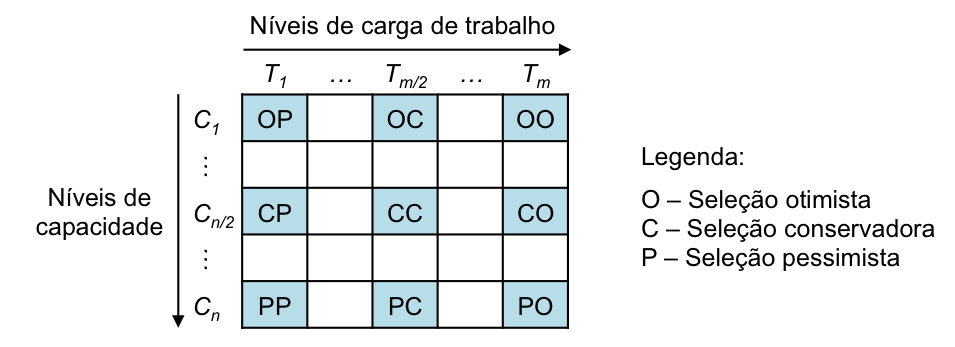
\includegraphics[trim = 20mm 5mm 20mm 10mm, scale=.6]{img/heuristicas2}
  \end{center}
  %\caption{\label{fig:heuristicas}Heurísticas de seleção utilizadas no processo de avaliação de capacidade.}
  \caption{\label{fig:heuristicas}Heurísticas para seleção de configurações e cargas de trabalho.}
\end{figure}

Na figura, as heurísticas são identificadas por diferentes pares de letras posicionados ao longo da matriz que representa o espaço de implantação. A primeira letra que identifica a heurística refere-se à tática usada na escolha da configuração (linha), enquanto a segunda letra refere-se à tática usada na escolha da carga de trabalho (coluna). Como pode-se observar, a tática otimista leva à escolha de configurações menores e cargas de trabalho maiores. Já a tática conservadora leva à escolha de configurações e cargas de trabalho de nível intermediário. Por fim, a tática pessimista leva à escolha de configurações maiores e cargas de trabalho menores.
 
No contexto do processo de avaliação de capacidade proposto neste trabalho, cada heurística de seleção fornece uma ``lógica'' diferente para exploração do espaço de implantação, servindo como base para a customização do processo com diferentes estratégias de avaliação. A acurácia e a eficiência do processo proposto, em particular, da abordagem de inferência de desempenho, utilizando cada uma das noves heurísticas de seleção mencionas acima, serão analisadas na próxima seção. 

%\subsection{Exemplo de Uso}

%\subsection{Implementação}

\section{Avaliação Experimental}\label{sec:experiments}

Esta seção descreve o experimento realizado como forma de verificação do processo de avaliação de capacidade apresentado anteriormente. Inicialmente, é apresentada a metodologia utilizada para a condução do experimento. Em seguida, são apresentados os resultados obtidos por cada uma das nove heurísticas de seleção propostas. Esses resultados são usados tanto para uma comparação qualitativa das heurísticas entre si, quanto para atestar
a eficiência do processo proposto e de sua abordagem de inferência de desempenho. 

É importante mencionar que o processo proposto foi implementado e está disponível na forma de uma ferramenta web,\footnote{\url{http://cloud-capacitor.herokuapp.com/}.} a qual foi utilizada para executar o experimento descrito a seguir. Devido a restrições de espaço, os detalhes da implementação do processo bem como de sua ferramenta de apoio estão fora do escopo deste artigo.

\subsection{Metodologia}

O experimento consistiu na realização de sessões de avaliação de
capacidade de uma aplicação web real (WordPress~\cite{wordpress}, um motor de construção 
e administração de \emph{blogs}) implantada em um provedor de nuvem IaaS público (Amazon EC2~\cite{ec2}). O WordPress foi implantado em duas camadas: uma para o banco de  dados MySQL, e outra para o servidor de aplicação, executada pelo servidor Apache HTTPD. Como balanceador de carga, foi utilizada uma máquina dedicada executando o servidor web Nginx. 


% A aplicação escolhida foi o WordPress \cite{wordpress}, um motor de construção 
% e administração de \emph{blogs}. Sua escolha foi motivada por ser uma aplicação
% bem conhecida, de utilização via web, ideal para implantação em ambiente de
% nuvem, e com componentes arquiteturais escaláveis. Além disso, o fluxo de 
% utilização típico da aplicação apresenta características bem diversificadas quanto ao uso
% de recursos de CPU e memória, rede, sistema de arquivos e banco de dados.

\begin{figure}[t]
  \begin{center}
    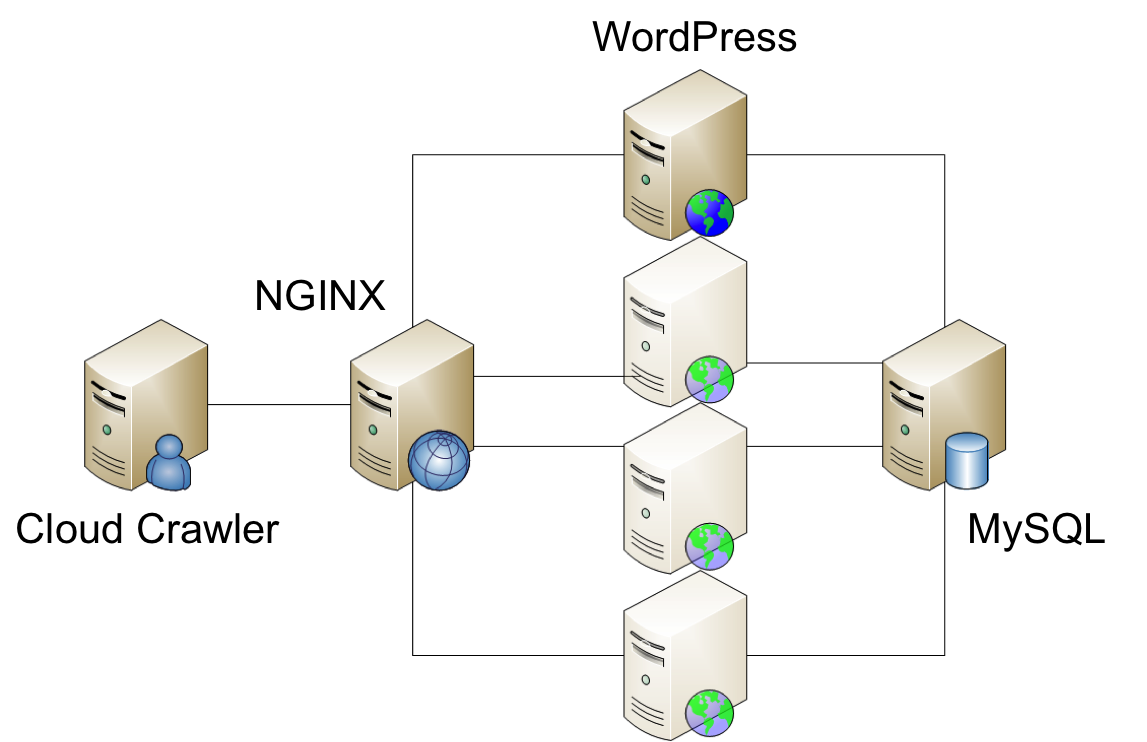
\includegraphics[scale=0.3]{img/ImplantacaoWordPress}
  \end{center}
  \caption{\label{fig:implantacao}Arquitetura de implantação do WordPress na Amazon EC2.}
\end{figure}

Devido a restrições de custo e tempo, o experimento limitou-se a variar 
apenas a camada de aplicação, usando de 1 a 4 servidores Apache executando o WordPress. 
A execução dos testes foi orquestrada pelo ambiente Cloud~Crawler~\cite{cunhacloud,cunha2013b},
que automatizou as tarefas de iniciar e parar todas as instâncias de máquinas virtuais, configurar 
o balanceador de carga de acordo com o número de instâncias testadas na camada de 
aplicação, iniciar e parar a execução dos testes, gerar as cargas de trabalho impostas à aplicação e, finalmente, coletar os dados de desempenho obtidos em cada teste. A Figura~\ref{fig:implantacao} mostra um panorama dessa arquitetura de implantação.

Para compor o espaço de implantação utilizado no experimento, 
foram escolhidos sete tipos de máquinas virtuais oferecidos pelo provedor Amazon EC2:
m3\_medium, m3\_large, m3\_xlarge, m3\_2xlarge, c3\_large, c3\_xlarge e
c3\_2xlarge. Para cada um desses tipos, foram criadas configurações
com 1, 2, 3 e 4 instâncias, levando a um total de 28 configurações diferentes no espaço de implantação,
divididas em duas categorias distintas, ``c3'' e ``c3''. As cargas de trabalho
para estes testes foram quantificadas em número de usuários concorrentes enviando
requisições ao WordPress. Foram definidas um total de 10 cargas de trabalho, representando
100, 200, 300, 400, 500, 600, 700, 800, 900 e 1000 usuários, respectivamente. 

De forma a estabelecer uma \emph{baseline} para validação e verificação das 
predições de desempenho realizada pelo process, foram coletados dados de desempenho do WordPress na nuvem para cada um dos 280 cenários possíveis, ou seja, foram efetivamente realizados testes de desempenho da aplicação para cada uma das 28 configurações criadas sob cada uma das 10 cargas de trabalho especificadas. A esse conjunto
de dados de execuções reais da aplicação foi dado o nome ``oráculo'' e à estratégia necessária para gerar esses todos esses dados foi dado o nome de heurística ``força bruta'' ({\em Brute Force -- BF}). As nove heurísticas propostas foram comparadas entre si e com a heurística BF, que representava o caso no qual nenhuma inferência foi feita quanto ao desempenho da aplicação. 

Cada teste de desempenho consistiu em executar o WordPress utilizando uma das 28 configurações definidas para o espaço de implantação e então submetê-lo a uma das 10 cargas de trabalho especificadas durante um período de 1 hora. Durante os testes, um gerador de carga criava a quantidade de usuários corresponde à carga de trabalho sendo avaliada, os quais disparavam a seguinte sequência de requisições à aplicação: efetuar \emph{logon}; inserir uma nova postagem; consultar a nova postagem; alterar a nova postagem; consultar postagens por palavra-chave; alterar uma postagem específica já existente; efetuar \emph{logoff}. 

A métrica de desempenho utilizada nos experimentos foi o {\em tempo de resposta total}, ou 
seja, o tempo total decorrido entre o envio da primeira requisição da sequência 
acima e o momento em que o usuário recebeu a resposta para última requisição da
sequência. Assim, para ser considerada como candidata para uma determinada carga de trabalho, uma configuração devia 
ser capaz de atender 90\% das sequências de requisições recebidas dos usuários em um tempo total igual ou inferior ao tempo informado na entrada do parâmetro SLA.

\subsection{Resultados}

\subsubsection{Eficiência}
Esta subseção apresenta os resultados de eficiência atingidos pelas heurísticas de seleção usadas 
no processo sob dois aspectos distintos: o custo total da avaliação e a quantidade de execuções realizadas por cada heurística. Esse custo foi calculado somando-se o preço da hora de utilização, conforme a tabela 
de preços do provedor na data realização dos testes, para cada uma das configurações 
para as quais foram realizadas execuções reais na nuvem. 

A Figura~\ref{fig:cost-time}(a) mostra o gráfico dos resultados obtidos pelas
nove heurísticas em termos de custo considerando SLAs 
entre 10 e 50 segundos. No topo do gráfico vê-se um linha horizontal
que representa a \emph{baseline} de comparação, que é o custo total obtido com a heurística BF. Como o custo total para execução da aplicação em todas
as combinações de configurações e cargas de trabalho é sempre o mesmo, independente
do SLA requerido, a curva do gráfico para essa heurística é sempre uma linha reta horizontal.

\begin{figure}[t]
\centering\footnotesize
  %trim option's parameter order: left bottom right top
  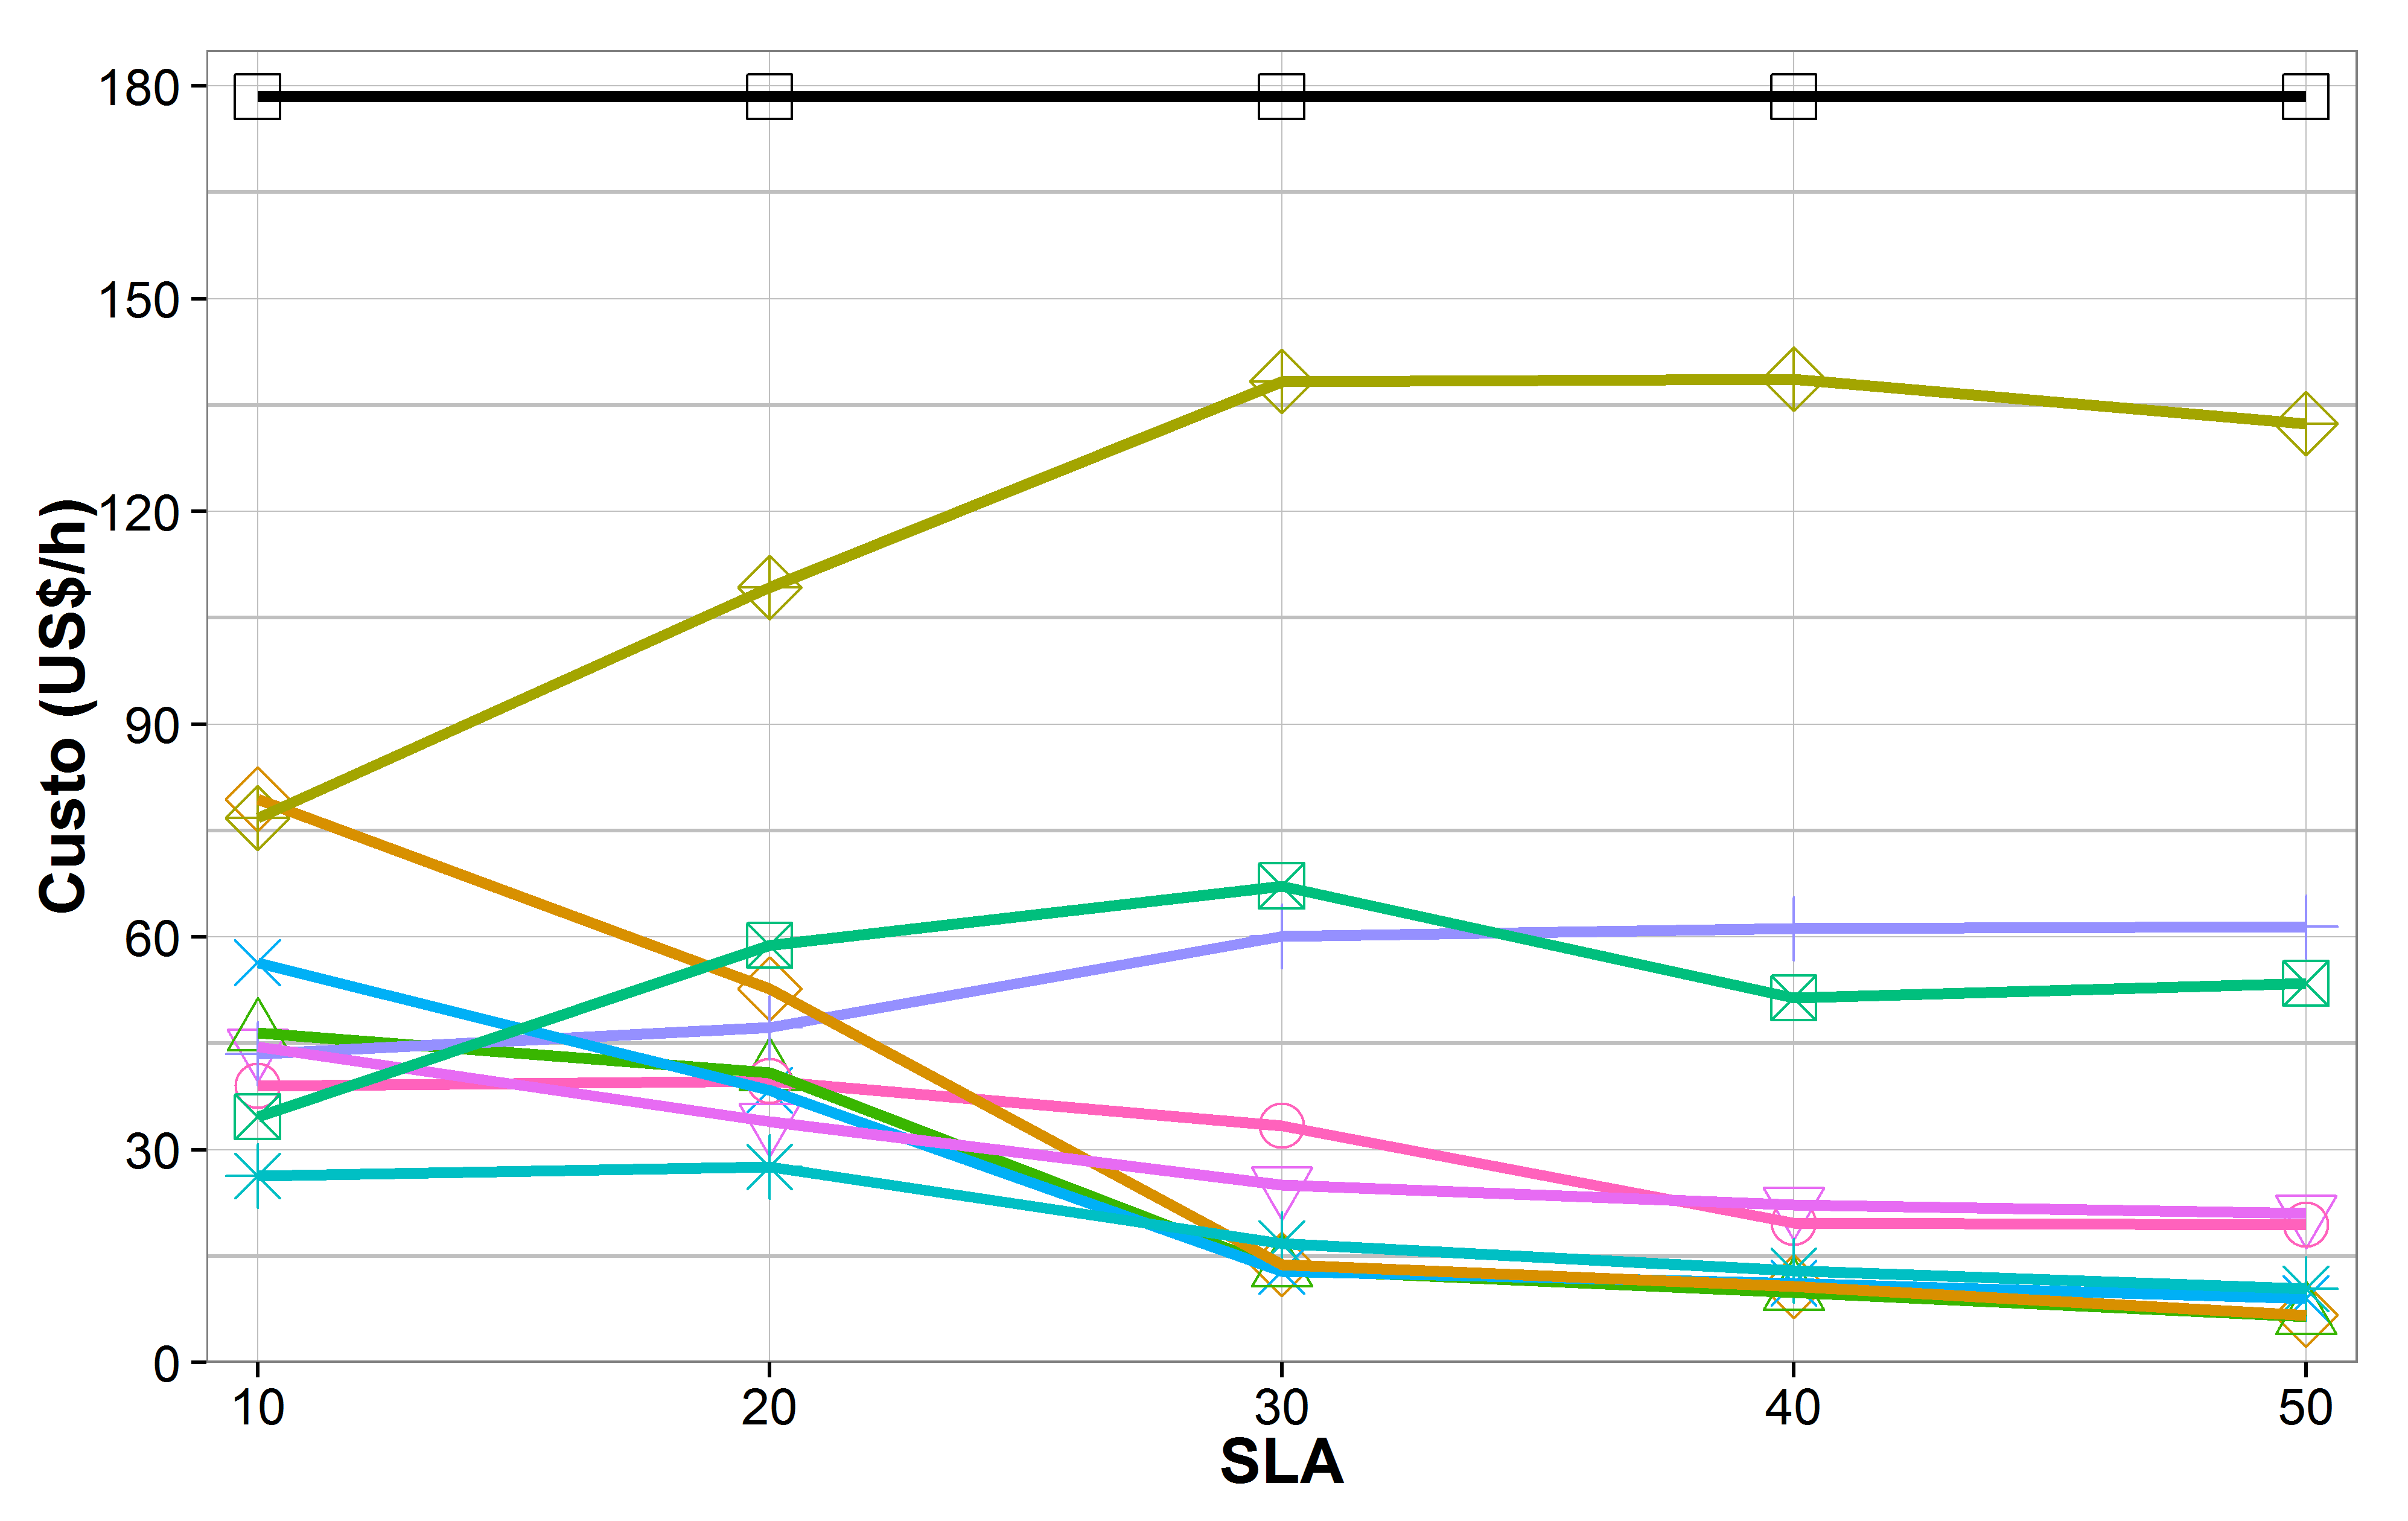
\includegraphics[trim = 12mm 10mm 8mm 20mm, width=0.49\textwidth]{img/graphic-cost-capacity.png}
  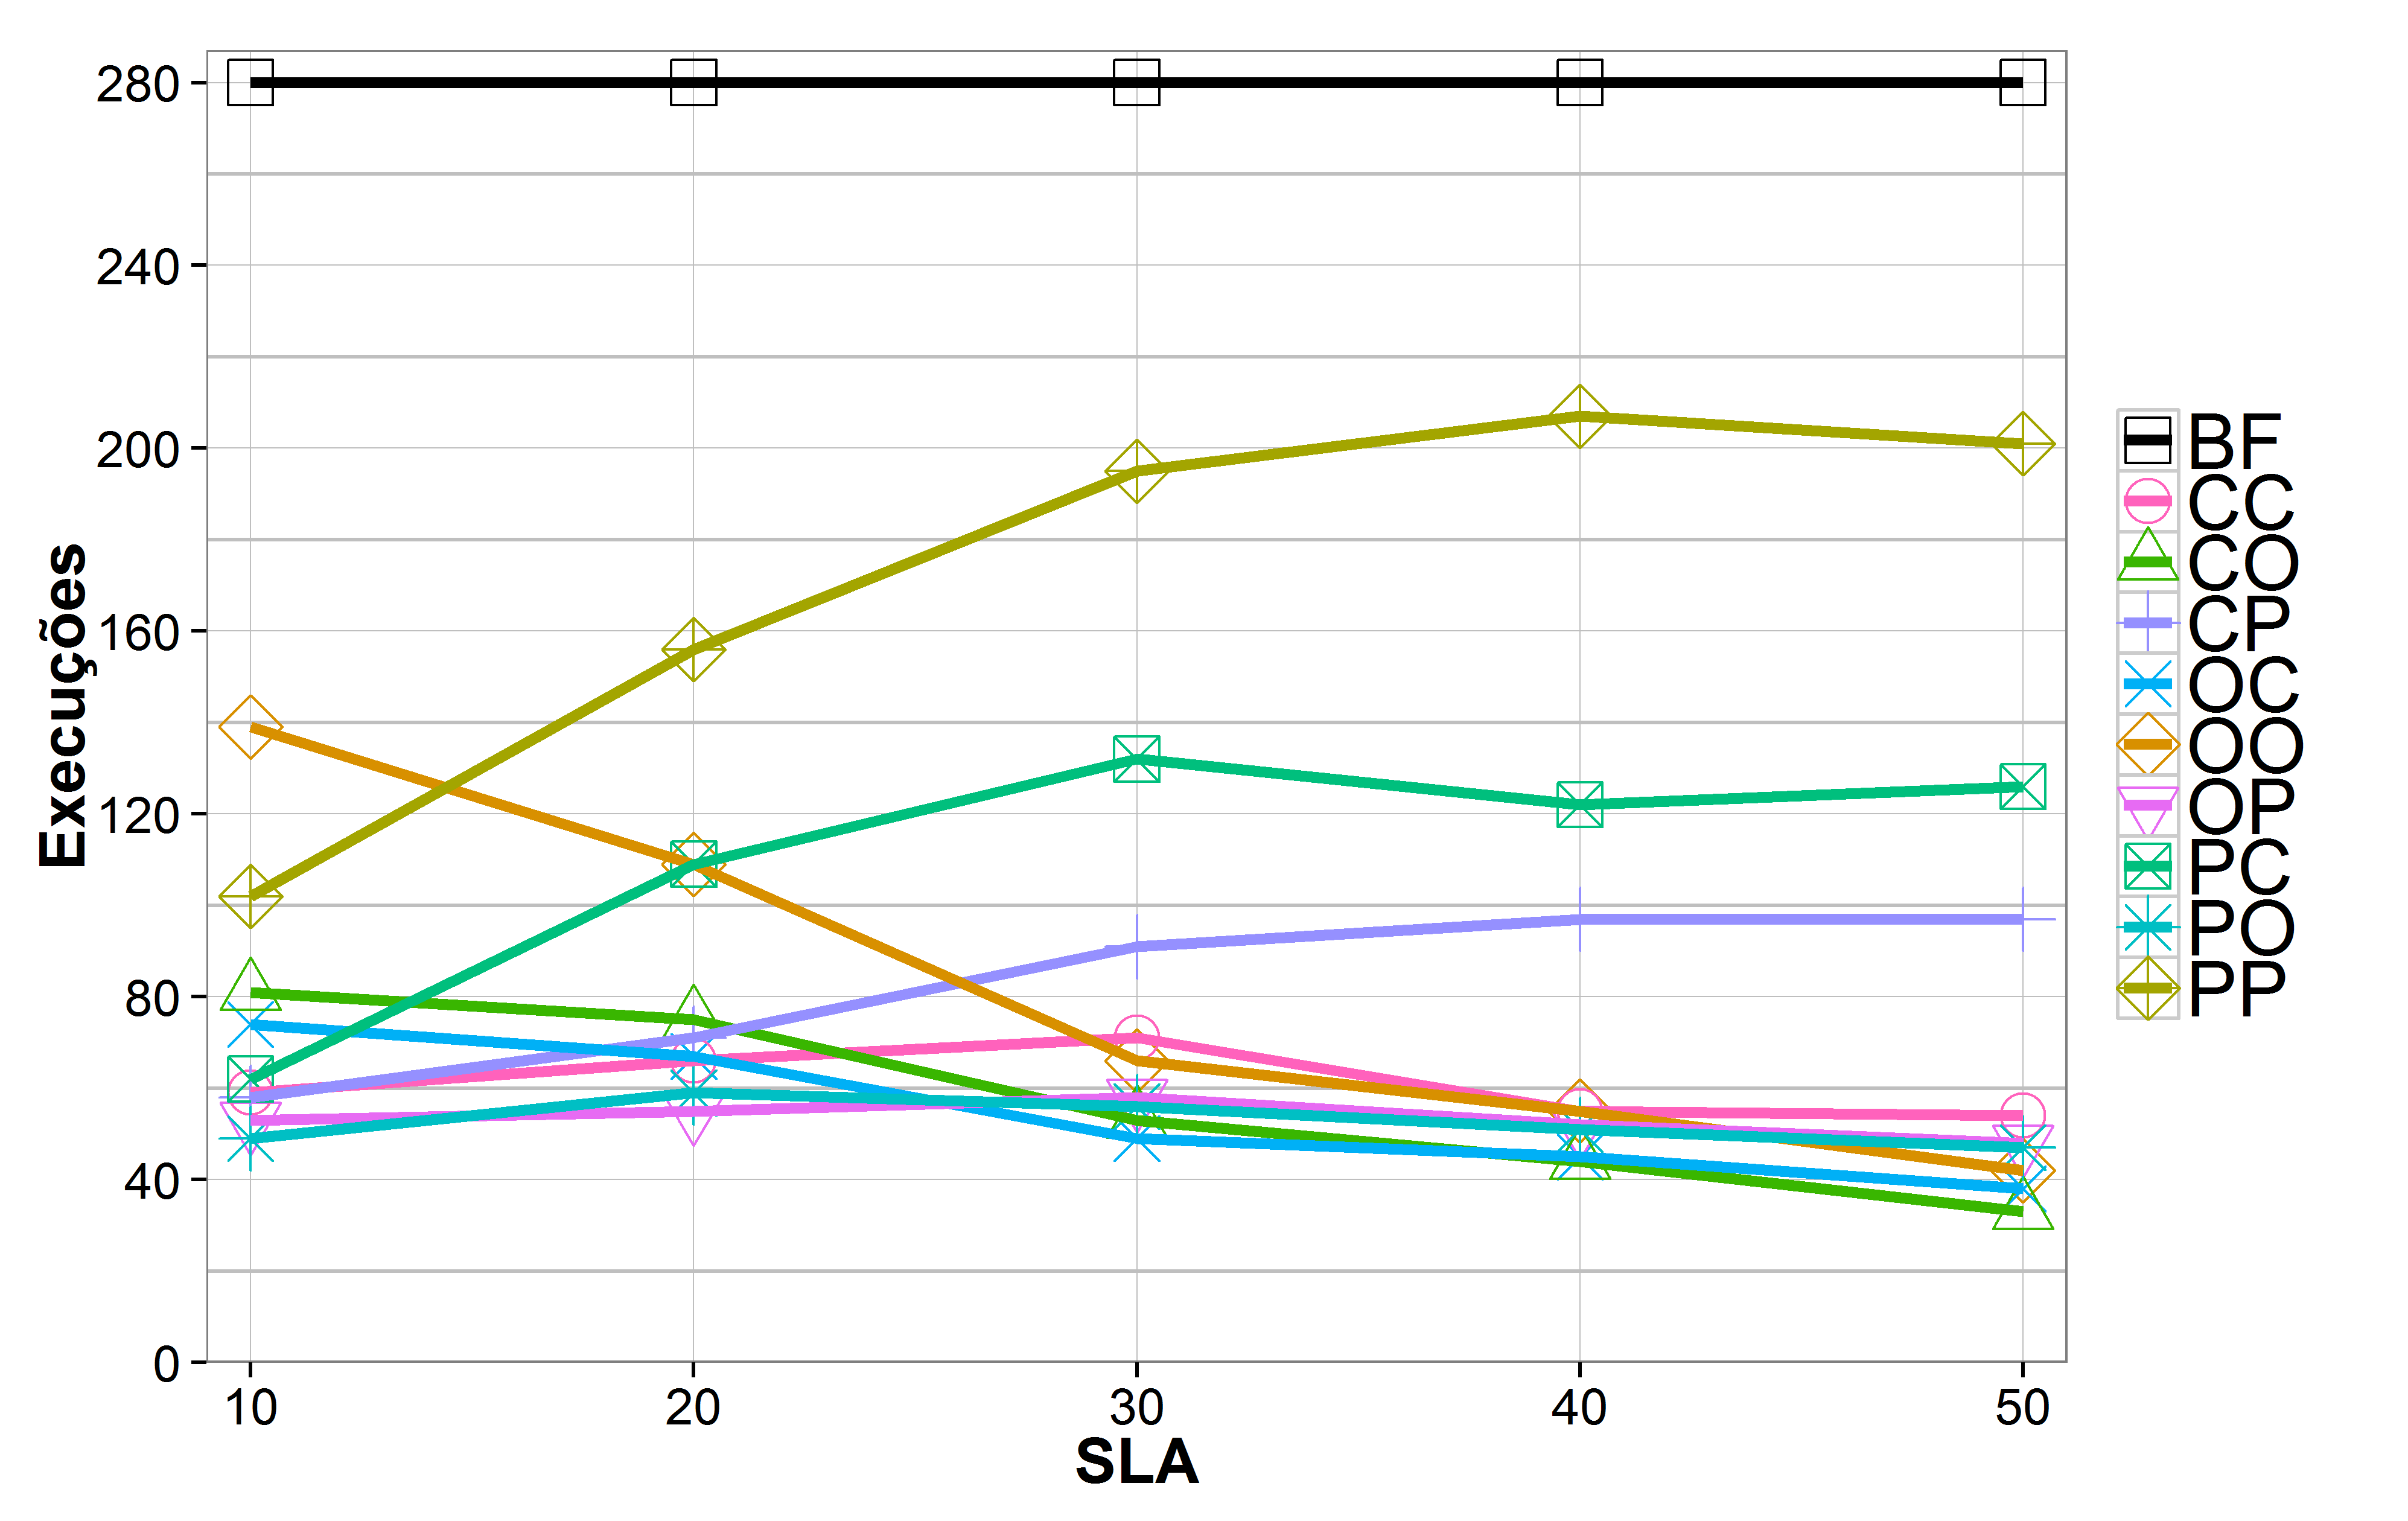
\includegraphics[trim = 12mm 10mm 8mm 20mm, width=0.49\textwidth]{img/graphic-time-capacity.png}
  \\~\\\hspace{0.24\textwidth}(a) \hfill (b) \hspace{0.24\textwidth}
  \caption{\label{fig:cost-time}Resultados de eficiência das heurísticas de seleção, em termos de custo (a) e número de execuções (b).}
\end{figure}

A análise do gráfico mostra que mesmo a heurística com o pior 
desempenho no que se refere ao custo já apresenta uma redução considerável 
em relação à heurística BF. Por outro lado, as melhores heurísticas chegam a 
representar uma economia da ordem de 96\% em comparação com o que seria gasto
com a execução de todas as combinações de configurações e cargas de trabalho.
Embora o comportamento das heurísticas varie em função do SLA, é possível notar
que quando a exigência do SLA é mais moderada, o comportamento de todas as heurísticas
se estabiliza, tornando possível identificar que algumas delas tendem a
ser mais econômicas que as outras. Ainda que não seja possível afirmar que uma só 
heurística seja a melhor em todas as situações, pode-se considerar que a heurística
Pessimista/Otimista (PO) se mostra como a mais econômica em geral. A heurística
Conservadora/Otimista (CO) merece atenção para os SLAs mais brandos, com os menores
custos absolutos nessas circunstâncias. 

Já Figura~\ref{fig:cost-time}(b) mostra o desempenho das heurísticas sob 
o aspecto da quantidade de execuções reais da aplicação no ambiente de
nuvem. A análise desse gráfico faz notar um número de execuções até 88\% menor em 
relação à heurística BF. Isso se reflete em menor tempo gasto no 
planejamento de capacidade e, consequentemente, menores custos, não só como já 
visto no que diz respeito à economia de horas de máquina, mas também de outros 
custos envolvidos em um projeto de software.

%\begin{figure}[t]
%  \begin{center}
%    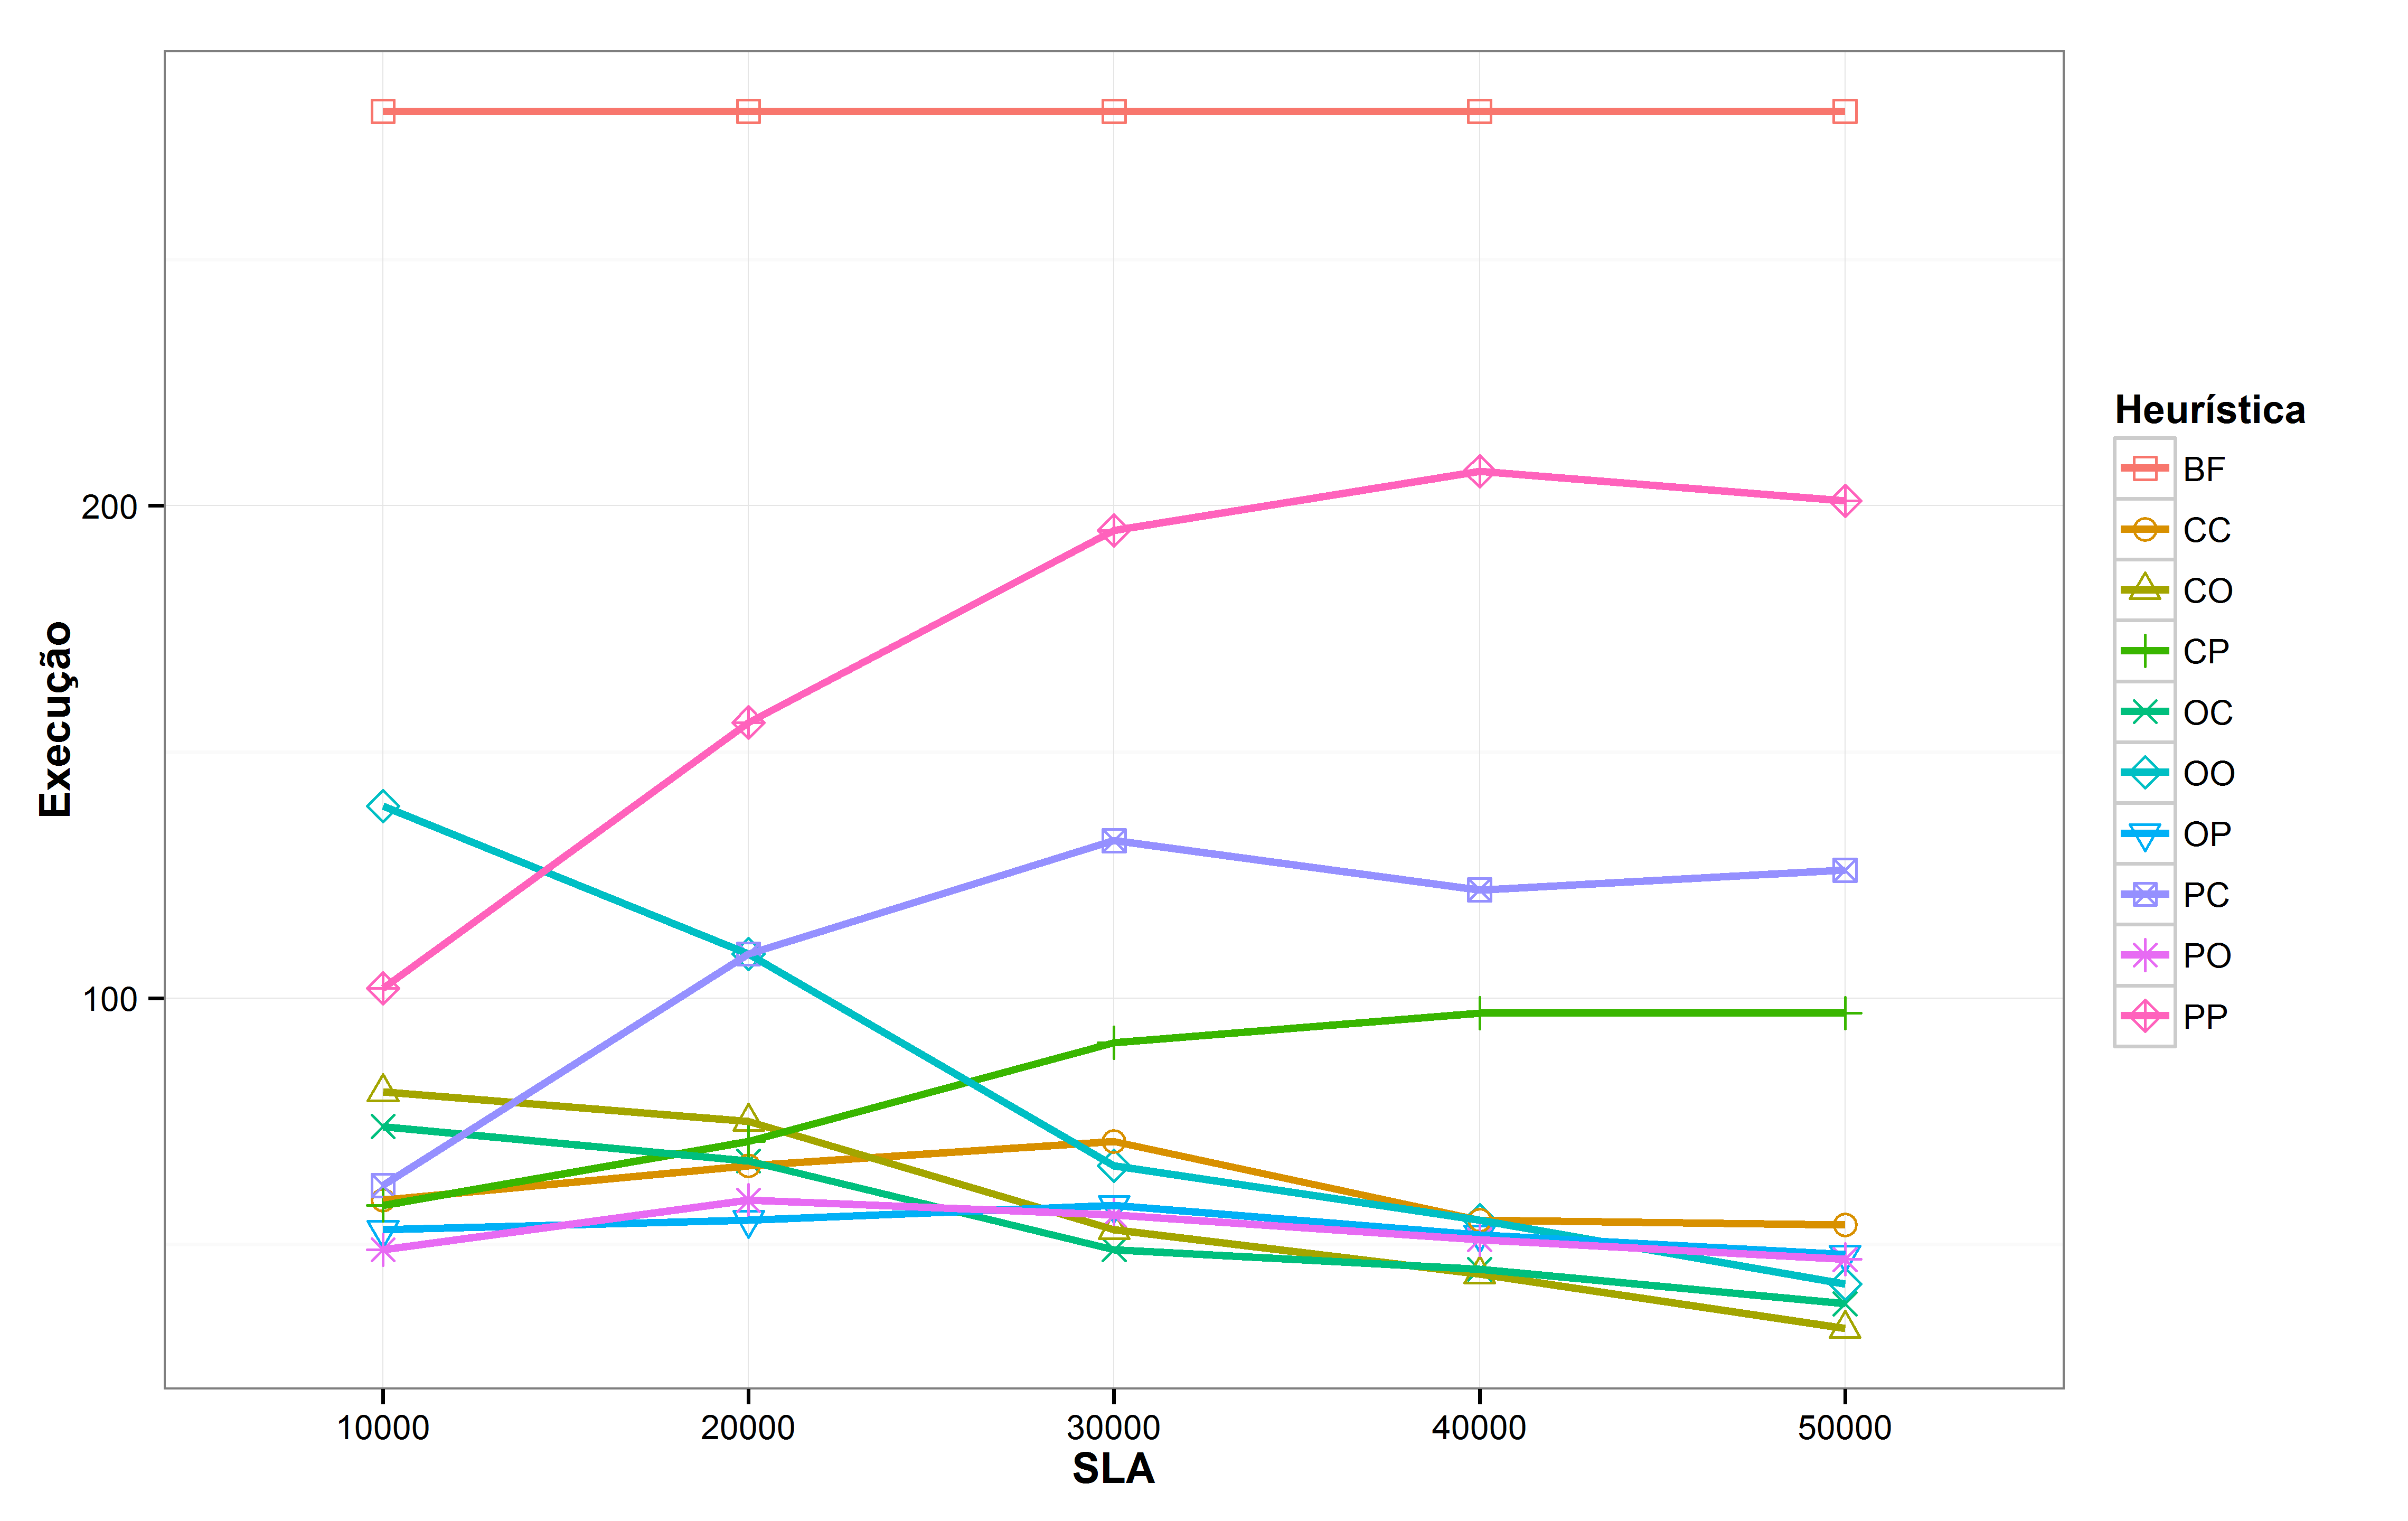
\includegraphics[scale=0.3]{img/ExecutionCount-Capacity}
%  \end{center}
%  \caption{\label{fig:eficiencia_execucoes}Avaliação da Eficiência do Número de Execuções das Heurísticas.}
%\end{figure}

Tanto no aspecto custo como no aspecto quantidade de execuções, nota-se que a
heurística Pessimista/Pessimista (PP) tem um desempenho bem inferior às demais heurísticas, exigindo muitas
execuções e, por isso, elevando muito o custo do planejamento de capacidade. As
heurísticas Pessimista/Conservadora (PC) e Conservadora/Pessimista (CP) ainda aparecem
um pouco descoladas do desempenho das outras heurísticas, embora com uma redução
em torno de 65\% no número de execuções.

Os menores números de execuções são atingidos pelas heurísticas Otimista/Conservadora (OC) 
e Conservadora/Otimista (CO), sob os SLAs mais brandos. Porém, como não se saem tão 
bem sob SLAs mais rígidos, como 10 segundos, a heurística PO
ganha destaque por ter comportamento mais estável, figurando entre as mais 
econômicas no aspecto de quantidade de execuções sob a maioria dos SLAs avaliados.

\subsubsection{Acurácia}

\unboldmath

Para medir a acurácia do processo de avaliação de capacidade, foram calculados os valores médios de \emph{Precision},
\emph{Recall} e \emph{F-Measure}~\cite{Baeza-Yates1999} para as predições realizadas por cada uma das heurísticas de seleção em todas as combinações de configurações e cargas de trabalho sob cada SLA, tomando como base o oráculo.  Nesse caso, os dados do oráculo foram utilizados para determinar se as configurações identificadas como candidatas e rejeitadas para cada carga de trabalho eram de fato verdadeiras (predições corretas) ou falsas (predições erradas).

Os valores dessas três métricas para uma carga de trabalho $i$, denotados por $P_{i}$, $R_{i}$ e $F_{i}$, respectivamente, são dados pelas seguintes fórmulas~\cite{Baeza-Yates1999}:

\begin{description}
\scriptsize
  \item[$P_{i}$] = $\dfrac{\emph{\# config. candidatas verdadeiras}}{\emph{\# config. candidatas verdadeiras}\,+\,\emph{\# config. candidatas falsas}}$
  \smallskip
  \item[$R_{i}$] = $\dfrac{\emph{\# config. candidatas verdadeiras}}{\emph{\# config. candidatas verdadeiras }\,+\,\emph{\# config. rejeitadas falsas}}$
  \smallskip
  \item[$F_{i}$] = $2\,\cdot\,\dfrac{\emph{$P_{i}$}\,\times\,\emph{$R_{i}$}}{\emph{$P_{i}$}\,+\,\emph{$R_{i}$}}$
\end{description}

%Considerando $m$ cargas de trabalho, as fórmulas para o cálculo das médias dos valores de \emph{Precision}, \emph{Recall} e \emph{F-Measure} de cada heurística de seleção para um dado SLA $s$,  denotados por $P\,(s)$, $R\,(s)$ e $F\,(s)$, respectivamente, são as seguintes: 
%
%
% \begin{description}
% \scriptsize
%   \item[\normalfont\emph{P~(s)}] = $\sum\limits_{i=1}^{m}\,P_{i,s}/m$
%   \smallskip
%   \item[\normalfont\emph{R~(s)}] = $\sum\limits_{i=1}^{m}\,R_{i,s}/m$
%   \smallskip
%   \item[\normalfont\emph{F~(s)}] = $\sum\limits_{i=1}^{m}\,F_{i,s}/m$
% \end{description}



\begin{table}[t]
   \centering\scriptsize
   \caption{\label{table:acuracia_capacidade}Resultados de acurácia das heurísticas de seleção.}
    \begin{tabular}{cm{.8em}m{.8em}m{1.4em}m{.8em}m{.8em}m{1.4em}m{.8em}m{.8em}m{1.4em}m{.8em}m{.8em}m{1.4em}m{.8em}m{.8em}m{.8em}}
    %\hline
    \toprule
     & \multicolumn{15}{c}{SLA (segundos)} \\
    \cline{2-16}
          & \multicolumn{3}{c}{10} & \multicolumn{3}{c}{20} & \multicolumn{3}{c}{30} & \multicolumn{3}{c}{40} & \multicolumn{3}{c}{50} \\
          \cline{2-16}
          \multicolumn{1}{c}{Heurísticas} & ~~~P     & ~~~R     & ~~~F     & ~~~P     & ~~~R     & ~~~F     & ~~~P     & ~~~R     & ~~~F     & ~~~P     & ~~~R     & ~~~F     & ~~~P     & ~~~R     & ~~~F \\
          %\hline
          \midrule          
    CC    & 1,00  & 1,00  & 1,00  & 1,00  & 1,00  & 1,00  & 1,00  & {\color{red}0,98}  & {\color{red}0,99}  & 1,00  & 1,00  & 1,00  & 1,00  & 1,00  & 1,00 \\
    CO    & 1,00  & 1,00  & 1,00  & 1,00  & 1,00  & 1,00  & {\color{red}0,99}  & 1,00  & {\color{red}0,99}  & 1,00  & 1,00  & 1,00  & 1,00  & 1,00  & 1,00 \\
    CP    & 1,00  & 1,00  & 1,00  & 1,00  & 1,00  & 1,00  & 1,00  & {\color{red}0,98}  & {\color{red}0,99}  & 1,00  & 1,00  & 1,00  & 1,00  & 1,00  & 1,00 \\
    OC    & 1,00  & 1,00  & 1,00  & 1,00  & 1,00  & 1,00  & {\color{red}0,99}  & {\color{red}0,99}  & {\color{red}0,99}  & 1,00  & 1,00  & 1,00  & 1,00  & 1,00  & 1,00 \\
    OO    & 1,00  & 1,00  & 1,00  & 1,00  & 1,00  & 1,00  & {\color{red}0,99}  & 1,00  & {\color{red}0,99}  & 1,00  & 1,00  & 1,00  & 1,00  & 1,00  & 1,00 \\
    OP    & 1,00  & 1,00  & 1,00  & 1,00  & 1,00  & 1,00  & 1,00  & {\color{red}0,98}  & {\color{red}0,99}  & 1,00  & 1,00  & 1,00  & 1,00  & 1,00  & 1,00 \\
    PC    & 1,00  & 1,00  & 1,00  & 1,00  & 1,00  & 1,00  & 1,00  & {\color{red}0,98}  & {\color{red}0,99}  & 1,00  & 1,00  & 1,00  & 1,00  & 1,00  & 1,00 \\
    PO    & 1,00  & 1,00  & 1,00  & 1,00  & 1,00  & 1,00  & {\color{red}0,99}  & 1,00  & {\color{red}0,99}  & 1,00  & 1,00  & 1,00  & 1,00  & 1,00  & 1,00 \\
    PP    & 1,00  & 1,00  & 1,00  & 1,00  & 1,00  & 1,00  & 1,00  & {\color{red}0,98}  & {\color{red}0,99}  & 1,00  & 1,00  & 1,00  & 1,00  & 1,00  & 1,00 \\
    %\hline
    \toprule
    \end{tabular}%
 \end{table}%

A Tabela~\ref{table:acuracia_capacidade} mostra os valores médios de $P_{i}$, $R_{i}$ e $F_{i}$ obtidos com cada heurística de seleção para os cinco níveis de SLA investigados. Nota-se que em apenas um dos cinco SLAs o processo deixou de obter 100\% de acurácia nas predições, apresentando uma taxa de erro inferior a 3\%. Uma investigação mais minuciosa dos dados de desempenho da aplicação na nuvem revelou que essa pequena perda na qualidade das predições foi devida a flutuações ocasionais no desempenho de algumas das máquinas virtuais disponibilizadas pelo provedor. Essas flutuações afetaram particularmente o desempenho da aplicação para o SLA de 30 segundos, refletindo em erros de predição. De fato, oscilações no desempenho da infraestrutura virtualizada oferecida por provedores de nuvem IaaS são relativamente comuns, como observados por \cite{iosup2011performance} e \cite{cunha2011investigating}. O impacto dessas flutuações nos resultados experimentais obtidos no contexto deste trabalho, porém, foi mínimo, afetando um único nível de SLA e mesmo assim mantendo o valor médio de \emph{F-Measure} (que estabelece uma média ponderada entre os valores de \emph{Precision} e \emph{Recall}~\cite{Baeza-Yates1999}) muito próximo a 99\%.


\section{Trabalhos Relacionados}\label{sec:related-work}

...


Para apoiar os usuários de nuvens IaaS no planejamento de capacidade, os trabalhos fazem uso de diferentes abordagens. Neste artigo serão expostos trabalhos que usam abordagens preditivas e empíricas. Na abordagem preditiva, a
aplicação alvo não é executada diretamente no ambiente onde se deseja implantá-la,~\cite{cloudharmony},~\cite{malkowski2010cloudxplor,li2011,jung2013cloudadvisor,fittkau2012cdosim} e~\cite{li2011cloudprophet}, fazem uso dessa abordagem. Já em~\cite{jayasinghe2012,silva2013cloudbench,cunhacloud} e~\cite{scheuner2014cloud} são apresentados trabalhos que utilizam a abordagem empírica, onde as aplicações alvo são implantadas na nuvem e então
submetidas a testes de carga.

As soluções de abordagem preditiva não requerem a alocação de recursos de nuvem para realizarem as predições, com
exceção do \textit{CloudProphet}, apresentado em~\cite{li2011cloudprophet}. Além disso, são soluções de baixa complexidade, com destaque para a apresentada em \cite{cloudharmony}, a qual permite que os testes sejam iniciados e que as pesquisas de resultados anteriores sejam realizadas através de uma interface amigável, sem a necessidade de intervenções do usuário. Por outro lado, essas soluções apresentam limitações na definição da aplicação alvo e dos
seus requisitos de desempenho,~\cite{malkowski2010cloudxplor,cloudharmony}, e os resultados das predições podem divergir dos valores reais. O que ficou evidenciado em~\cite{fittkau2012cdosim}, onde os valores da CPU simulada, em comparação com os valores da CPU medida, divergiram na ordem de 30~\%.

Essas limitações, apresentadas pelas soluções de abordagem preditiva, são superadas pelas soluções de abordagem empírica que permitem ao usuário definir os componentes da aplicação e os seus resultados são reflexo da execução real da aplicação alvo. Como exemplo de uma solução de abordagem empírica, em~\cite{cunhacloud} o usuário pode definir toda a pilha de componentes da aplicação alvo, todos cenários utilizados na avaliação de desempenho, as demandas que serão submetidas a cada um dos cenários e o critério que define se o cenário suportou a demanda, ou seja, o SLA. Da mesma forma, as soluções apresentadas em~\cite{jayasinghe2012,silva2013cloudbench,scheuner2014cloud}, possuem os seus mecanismos para a realização dessas definições. Porém, elas precisam executar cada um dos cenários definidos pelo usuário e não fazem uso de resultados anteriores para evitar a execução de testes que claramente poderiam ser evitados.

Nesse contexto, o novo processo apresentado neste trabalho segue uma abordagem híbrida, combinando aspectos positivos das abordagens preditiva e empírica. Por exemplo, em uma situação na qual uma demanda é submetida à aplicação que está sendo executada em uma máquina virtual com baixo poder computacional, o processo pode afirmar que essa mesma demanda pode ser atendida por máquinas com perfis computacionais mais robustos, e dessa forma diminuir o número de execuções e consequentemente os custos da avaliação.


\section{Conclusão}\label{sec:conclusion}

O processo de inferência de desempenho se mostrou uma solução eficaz, com acurácia medida em cerca de 99\%.
Além disso, mostrou-se também muito eficiente, apresentando redução de custo de até 96\% e redução do tempo
de execução de até 88, em relação à execução total de todas as combinações de cargas de trabalho e configurações.

Há oportunidades de extensão deste trabalho na criação de novas heurísticas, com uso de dados de comprometimento
de CPU e memória, por exemplo; estudo do impacto da flutuação de desempenho da nuvem sobre a acurácia do processo;
e investigação do uso da inferência de desempenho no planejamento de capacidade para outros perfis de aplicações.

%\section*{Agradecimentos}
%Este trabalho é parcialmente financiado pelo Conselho Nacional de Desenvolvimento Científico e Tecnológico (CNPq), através dos processos 311617/2011-5 e 487174/2012-7.

\bibliographystyle{sbc}
\bibliography{principal-capacitor}
\end{document}